% Options for packages loaded elsewhere
\PassOptionsToPackage{unicode}{hyperref}
\PassOptionsToPackage{hyphens}{url}
\documentclass[
  ignorenonframetext,
  aspectratio=169,
]{beamer}
\newif\ifbibliography
\usepackage{pgfpages}
\setbeamertemplate{caption}[numbered]
\setbeamertemplate{caption label separator}{: }
\setbeamercolor{caption name}{fg=normal text.fg}
\beamertemplatenavigationsymbolsempty
% remove section numbering
\setbeamertemplate{part page}{
  \centering
  \begin{beamercolorbox}[sep=16pt,center]{part title}
    \usebeamerfont{part title}\insertpart\par
  \end{beamercolorbox}
}
\setbeamertemplate{section page}{
  \centering
  \begin{beamercolorbox}[sep=12pt,center]{section title}
    \usebeamerfont{section title}\insertsection\par
  \end{beamercolorbox}
}
\setbeamertemplate{subsection page}{
  \centering
  \begin{beamercolorbox}[sep=8pt,center]{subsection title}
    \usebeamerfont{subsection title}\insertsubsection\par
  \end{beamercolorbox}
}
% Prevent slide breaks in the middle of a paragraph
\widowpenalties 1 10000
\raggedbottom
\AtBeginPart{
  \frame{\partpage}
}
\AtBeginSection{
  \ifbibliography
  \else
    \frame{\sectionpage}
  \fi
}
\AtBeginSubsection{
  \frame{\subsectionpage}
}
\usepackage{iftex}
\ifPDFTeX
  \usepackage[T1]{fontenc}
  \usepackage[utf8]{inputenc}
  \usepackage{textcomp} % provide euro and other symbols
\else % if luatex or xetex
  \usepackage{unicode-math} % this also loads fontspec
  \defaultfontfeatures{Scale=MatchLowercase}
  \defaultfontfeatures[\rmfamily]{Ligatures=TeX,Scale=1}
\fi
\usepackage{lmodern}
\ifPDFTeX\else
  % xetex/luatex font selection
\fi
% Use upquote if available, for straight quotes in verbatim environments
\IfFileExists{upquote.sty}{\usepackage{upquote}}{}
\IfFileExists{microtype.sty}{% use microtype if available
  \usepackage[]{microtype}
  \UseMicrotypeSet[protrusion]{basicmath} % disable protrusion for tt fonts
}{}
\makeatletter
\@ifundefined{KOMAClassName}{% if non-KOMA class
  \IfFileExists{parskip.sty}{%
    \usepackage{parskip}
  }{% else
    \setlength{\parindent}{0pt}
    \setlength{\parskip}{6pt plus 2pt minus 1pt}}
}{% if KOMA class
  \KOMAoptions{parskip=half}}
\makeatother
\usepackage{longtable,booktabs,array}
\usepackage{caption}
\captionsetup[table]{skip=6pt}
\newcounter{none} % for unnumbered tables
\usepackage{calc} % for calculating minipage widths
\usepackage{caption}
% Make caption package work with longtable
\makeatletter
\def\fnum@table{\tablename~\thetable}
\makeatother
\usepackage{graphicx}
\makeatletter
\newsavebox\pandoc@box
\newcommand*\pandocbounded[1]{% scales image to fit in text height/width
  \sbox\pandoc@box{#1}%
  \Gscale@div\@tempa{\textheight}{\dimexpr\ht\pandoc@box+\dp\pandoc@box\relax}%
  \Gscale@div\@tempb{\linewidth}{\wd\pandoc@box}%
  \ifdim\@tempb\p@<\@tempa\p@\let\@tempa\@tempb\fi% select the smaller of both
  \ifdim\@tempa\p@<\p@\scalebox{\@tempa}{\usebox\pandoc@box}%
  \else\usebox{\pandoc@box}%
  \fi%
}
% Set default figure placement to htbp
\def\fps@figure{htbp}
\makeatother
\setlength{\emergencystretch}{3em} % prevent overfull lines
\providecommand{\tightlist}{%
  \setlength{\itemsep}{0pt}\setlength{\parskip}{0pt}}
% Auto-generated by infrastructure/rendering/_pdf_latex_helpers.py::extract_math_font_preamble.
% Minimal header passed to Pandoc via -H so Beamer slides pick up the same math font
% as the combined-PDF path. Adjust the manuscript's preamble.md to change the font globally.
\usepackage{unicode-math}
\setmathfont{latinmodern-math.otf}

% Manuscript macro/package fallbacks (newcommand -> providecommand).
% Core mathematics
\usepackage{amsmath}
\usepackage{amssymb}
% Document layout
% Tables
\usepackage{booktabs}
% Caption styling (booktabs already loaded above). Small caption font with a
% bold label ("Figure 1", "Table 2") gives the math/figure-heavy layout a
% consistent, journal-like caption rhythm without fighting pandoc-crossref —
% pandoc emits standard \caption{}, and caption/captionsetup only restyle it.
% ── Theorem environments ─────────────────────────────────────────────────
% amsthm is loaded above. The FedGVI<->Friston bridge is stated as a small
% number of theorems/definitions/lemmas/propositions/corollaries; sharing one
% counter (definition/lemma/proposition/corollary all step the `theorem`
% counter) gives a single monotone numbering 1, 2, 3, ... across all kinds, so
% authors can reference them as Theorem 1, Definition 2, Corollary 3 without a
% per-kind counter drifting out of order. Plain style for theorem-like results,
% definition style (upright body) for definitions.
% (algorithm2e intentionally not loaded: this manuscript states results as
% numbered amsthm Theorems/Definitions, not algorithm2e pseudocode.)
% Code listings
\usepackage{listings}
% Typography and formatting
% (siunitx intentionally not loaded: no \SI/\num units appear in this manuscript.)
% Cross-references and citations
% (cleveref and titlesec intentionally not loaded: unavailable in this TeX tree
% and not required. Cross-references resolve through pandoc-crossref's own
% \ref-style names — no \cref appears — and section heading styling falls back
% to the pandoc/LaTeX defaults.)
% ── TeX Live Basic-compatible mono font for code listings ────────────
% Latin Modern Mono is bundled with TeX Live Basic and keeps the manuscript
% renderable on minimal TeX installations. Mathematical Unicode coverage is
% provided separately by Latin Modern Math below, so the code font does not
% need a private JuliaMono installation.
%
% Use the TeX font filename rather than the system-family name: the minimal
% TeX Live fontconfig database may not register the OpenType family even though
% kpsewhich can resolve the bundled files.
% Math font for unicode-math: Latin Modern Math (TeX Live) has full BMP
% coverage including U+2223 (\mid), U+226A/226B (\ll/\gg), and the Greek/
% blackboard letters used in equations. Without an explicit \setmathfont,
% unicode-math falls back to lmroman text font which lacks several glyphs
% and emits "Missing character" warnings on every \mid in math mode.

% Slide layout defaults for warning-clean scientific decks.
\usepackage{etoolbox}
\IfFileExists{xurl.sty}{\usepackage{xurl}}{}
\IfFileExists{seqsplit.sty}{\usepackage{seqsplit}}{\newcommand{\seqsplit}[1]{#1}}
\protected\def\breakseq#1{\seqsplit{#1}}
\protected\def\breaktt#1{\begingroup\ttfamily\seqsplit{#1}\endgroup}
\setlength{\emergencystretch}{6em}
\tolerance=5000
\hbadness=10000
\hfuzz=1pt
\setlength{\tabcolsep}{2pt}
\AtBeginEnvironment{longtable}{\tiny\renewcommand{\arraystretch}{0.86}\setlength{\tabcolsep}{1pt}}
\AtBeginEnvironment{tabular}{\tiny\renewcommand{\arraystretch}{0.86}\setlength{\tabcolsep}{1pt}}
\AtBeginEnvironment{equation}{\tiny}
\AtBeginEnvironment{equation*}{\tiny}
\AtBeginEnvironment{align}{\tiny}
\AtBeginEnvironment{align*}{\tiny}
\AtBeginEnvironment{itemize}{\footnotesize}
\AtBeginEnvironment{enumerate}{\footnotesize}
\AtBeginEnvironment{description}{\footnotesize}
\setbeamerfont{caption}{size=\tiny}
\setbeamerfont{caption name}{size=\tiny}
\setbeamerfont{normal text}{size=\small}
\setbeamerfont{frametitle}{size=\small}
\setbeamerfont{section title}{size=\footnotesize}
\setbeamerfont{subsection title}{size=\footnotesize}
\setbeamertemplate{section page}{%
  \centering
  \begin{beamercolorbox}[sep=12pt,center,wd=\paperwidth]{section title}
    \parbox{0.86\paperwidth}{\centering\usebeamerfont{section title}\insertsection\par}
  \end{beamercolorbox}
}
\setbeamertemplate{subsection page}{%
  \centering
  \begin{beamercolorbox}[sep=8pt,center,wd=\paperwidth]{subsection title}
    \parbox{0.86\paperwidth}{\centering\usebeamerfont{subsection title}\insertsubsection\par}
  \end{beamercolorbox}
}
\setlength{\abovecaptionskip}{2pt}
\setlength{\belowcaptionskip}{0pt}

% Natbib and cross-reference fallbacks — slides don't load natbib
% or cleveref, but combined-PDF manuscript prose may emit these
% commands. The fallback renders citations as a bracketed key list
% and cross-references as detokenized labels so slides don't fail on
% undefined control sequences or raw underscores. \providecommand is
% a no-op if packages load later.
\providecommand{\citep}[1]{[#1]}
\providecommand{\citet}[1]{#1}
\providecommand{\citealp}[1]{#1}
\providecommand{\citeauthor}[1]{#1}
\providecommand{\citeyear}[1]{#1}
\providecommand{\cref}[1]{\texttt{\detokenize{#1}}}
\providecommand{\Cref}[1]{\texttt{\detokenize{#1}}}
\providecommand{\crefrange}[2]{\texttt{\detokenize{#1}}--\texttt{\detokenize{#2}}}
\providecommand{\Crefrange}[2]{\texttt{\detokenize{#1}}--\texttt{\detokenize{#2}}}
\providecommand{\paragraph}[1]{\textbf{#1}\ }

% Opt-in accessible presentation profile.
\setbeamerfont{normal text}{size*={20pt}{24pt}}
\setbeamerfont{frametitle}{size*={28pt}{32pt}}
\setbeamerfont{section title}{size*={28pt}{32pt}}
\setbeamerfont{subsection title}{size*={28pt}{32pt}}
\setbeamerfont{caption}{size*={16pt}{19pt}}
\setbeamerfont{caption name}{size*={16pt}{19pt}}
\setbeamerfont{itemize/enumerate body}{size*={20pt}{24pt}}
\setbeamerfont{itemize/enumerate subbody}{size*={20pt}{24pt}}
\setbeamerfont{itemize/enumerate subsubbody}{size*={20pt}{24pt}}
\setbeamerfont{itemize item}{size*={20pt}{24pt}}
\setbeamerfont{itemize subitem}{size*={20pt}{24pt}}
\setbeamerfont{itemize subsubitem}{size*={20pt}{24pt}}
\setbeamerfont{description body}{size*={20pt}{24pt}}
\setbeamerfont{description item}{size*={20pt}{24pt}}
\setbeamerfont{quote}{size*={20pt}{24pt}}
\setbeamerfont{quotation}{size*={20pt}{24pt}}
\AtBeginEnvironment{longtable}{\fontsize{20pt}{24pt}\selectfont}
\AtBeginEnvironment{tabular}{\fontsize{20pt}{24pt}\selectfont}
\AtBeginEnvironment{equation}{\fontsize{20pt}{24pt}\selectfont}
\AtBeginEnvironment{equation*}{\fontsize{20pt}{24pt}\selectfont}
\AtBeginEnvironment{align}{\fontsize{20pt}{24pt}\selectfont}
\AtBeginEnvironment{align*}{\fontsize{20pt}{24pt}\selectfont}
\AtBeginEnvironment{itemize}{\fontsize{20pt}{24pt}\selectfont}
\AtBeginEnvironment{enumerate}{\fontsize{20pt}{24pt}\selectfont}
\AtBeginEnvironment{description}{\fontsize{20pt}{24pt}\selectfont}
\AtBeginDocument{\usebeamerfont{normal text}}
\newlength{\AFSlideTableWidth}
% The fixed footer reservation is calibrated with the semantic seven-line regular-body budget.
\setbeamertemplate{footline}{%
  \leavevmode\vbox{%
    \hbox{%
      \begin{beamercolorbox}[wd=\paperwidth,ht=16pt,dp=3pt,center]{author in head/foot}%
        \fontsize{16pt}{19pt}\selectfont Untagged PDF derivative \textbar\ \href{../web/index.html}{HTML reader}%
      \end{beamercolorbox}%
    }%
    \vskip6pt%
  }%
}
% Accessible footer reserved height: 25pt.

\newtheorem{proposition}{Proposition}
\newtheorem{hypothesis}{Hypothesis}
\newtheorem{remark}[theorem]{Remark}
\newtheorem{axiom}{Axiom}
\newtheorem{property}{Property}
\usepackage{bookmark}
\IfFileExists{xurl.sty}{\usepackage{xurl}}{} % add URL line breaks if available
\urlstyle{same}
% fallback for those not using the hyperref driver hyperxmp:
\makeatletter
\@ifundefined{xmpquote}{\newcommand{\xmpquote}[1]{#1}}{}
\makeatother
\hypersetup{
  hidelinks,
  pdfcreator={LaTeX via pandoc}}

\author{\texorpdfstring{}{}}
\date{}

\begin{document}

\begin{frame}{Signed accuracy contrasts over acuity and colony size}
\protect\phantomsection\label{sec:results-sensitivity}
Studies 1--7 fix specific parameter configurations (sensor acuity and
colony size) to isolate mechanistic claims.
\end{frame}

\begin{frame}{Signed accuracy contrasts\ldots{} (part 2)}
Study 8 asks how the communicating-minus- isolated and
hierarchical-minus-flat accuracy contrasts vary across a systematic
two-dimensional sweep.
\end{frame}

\begin{frame}{Signed accuracy contrasts\ldots{} (part 3)}
This estimand-first formulation makes sign changes visible without
presuming that either architecture is uniformly advantageous.

We sweep sensor acuity \(\kappa \in \{0.40, 0.55, 0.70, 0.85, 0.95\}\)
and colony size \(n \in \{2, 4, 6, 8, 10\}\), evaluating two systems:
\end{frame}

\begin{frame}{Signed accuracy contrasts\ldots{} (part 4)}
\begin{itemize}
\tightlist
\item
  \textbf{Belief sharing} (Study 1 architecture) --- accuracy gap =
  communicating minus isolated mean accuracy;
\item
  \textbf{Hierarchical POMDP} (Study 6 architecture) --- accuracy gap =
  hierarchical minus flat location accuracy.
\end{itemize}
\end{frame}

\begin{frame}{Signed accuracy contrasts\ldots{} (part 5)}
Each cell averages \(n_{\text{trials}} = 20\) independent trials to
reduce Monte-Carlo noise at the cell level.
\end{frame}

\begin{frame}{Signed accuracy contrasts\ldots{} (part 6)}
The resulting heatmaps (fig.~29) show the
accuracy gap for both systems as a function of acuity and colony size.
The signed scale is centered on zero: brown cells encode positive gaps,
blue cells encode negative gaps, and the neutral midpoint encodes zero.
\end{frame}

\begin{frame}{Signed accuracy contrasts\ldots{} (part 7)}
Every cell also prints its signed value, so the direction remains
explicit without color. Hatching identifies only the declared
\(|\mathrm{gap}| \le 0.05\) display band; it is not an unreliability
flag, confidence interval, significance test, or proof of zero effect.
\end{frame}

\begin{frame}{Signed accuracy contrasts\ldots{} (part 8)}
Across the grid the following patterns hold:
\end{frame}

\begin{frame}{Pattern 1: low-to-moderate acuity}
\protect\phantomsection\label{pattern-1-low-to-moderate-acuity}
\textbf{Positive communicating-minus-isolated contrasts occur at
low-to-moderate acuity.} The accuracy gap peaks in the second-lowest
acuity row, where observations carry some signal but no single sentinel
resolves the location alone.
\end{frame}

\begin{frame}{Pattern 1: low-to-moderate\ldots{} (part 2)}
It remains positive across the two lowest-acuity rows for colonies of at
least four agents in the declared grid.

Near ceiling acuity the gap approaches zero because isolated agents
already solve most trials in the declared task.
\end{frame}

\begin{frame}{Pattern 2: a colony-size floor}
\protect\phantomsection\label{pattern-2-a-colony-size-floor}
\textbf{Colony size acts through a floor, not a smooth slope.} The
two-agent column shows an exactly zero belief-sharing gap at every
acuity. Under self-exclusion (``agents do not hear themselves''), each
member hears exactly one incoming belief, so the heard consensus adds no
pooled evidence.
\end{frame}

\begin{frame}{Pattern 2: a colony-size\ldots{} (part 2)}
Colonies of four or more show the positive low-acuity contrast within
this grid.
\end{frame}

\begin{frame}{Pattern 3: a conditional hierarchical contrast}
\protect\phantomsection\label{pattern-3-a-conditional-hierarchical-contrast}
\textbf{The hierarchical contrast changes with acuity and colony size.}
Negative hierarchical-minus-flat location-accuracy gaps occur across the
lower-acuity rows, including colonies larger than two agents.
\end{frame}

\begin{frame}{Pattern 3: a conditional\ldots{} (part 2)}
The higher-acuity rows are near zero outside the two-agent column;
positive cells are confined to that column in this grid. This
conditional pattern does not establish a general hierarchical accuracy
advantage,
\end{frame}

\begin{frame}{Pattern 3: a conditional\ldots{} (part 3)}
and the per-study paired location contrast remains a separate estimate
under its own trial and seed budget.
\end{frame}

\begin{frame}{Pattern 3: a conditional\ldots{} (part 4)}
The full parameter grid and protocol details are in the supplement
(sec.~14.14). A native-unit cross-study overview of
the headline metrics across all 9 studies is shown in
fig.~30.
\end{frame}

\begin{frame}{Pattern 3: a conditional\ldots{} (part 5)}
Read the page-compatible composition down the full left column and then
down the right: Panel A contains the six accuracy rows, Panel B at upper
right the two information or free-energy rows, and Panel C at lower
right the single recovery row. Each study appears once, in its
applicable native-unit panel.
\end{frame}

\begin{frame}{Pattern 3: a conditional\ldots{} (part 6)}
\begin{figure}
\centering
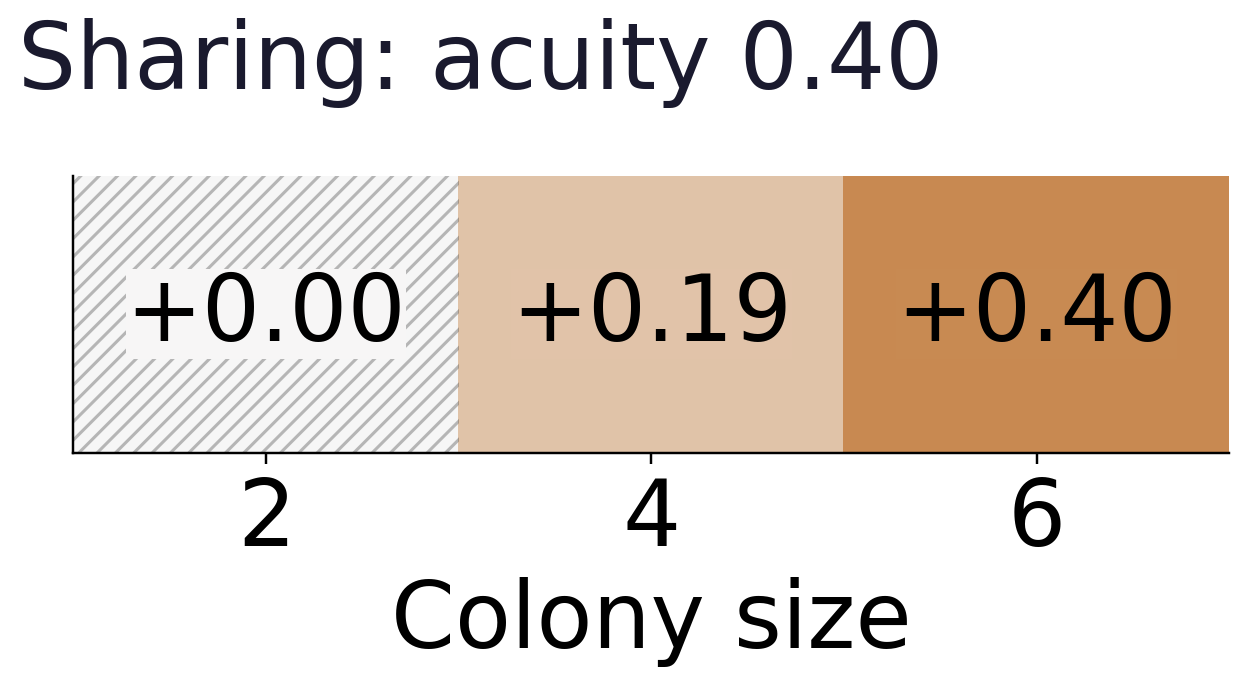
\includegraphics[keepaspectratio,width=0.98\linewidth,height=0.8\textheight,alt={Sharing, acuity 0.40: every signed accuracy gap in the displayed colony-size cells; common symmetric color scale and display-band hatch.}]{../figures/sensitivity_heatmap.slide-sharing-acuity-1-columns-1-3.png}
\refstepcounter{figure}\label{fig:sensitivity-heatmap-slide-panel-1}
\end{figure}
\end{frame}

\begin{frame}{Pattern 3: a conditional\ldots{} (part 7)}
\begin{figure}
\centering
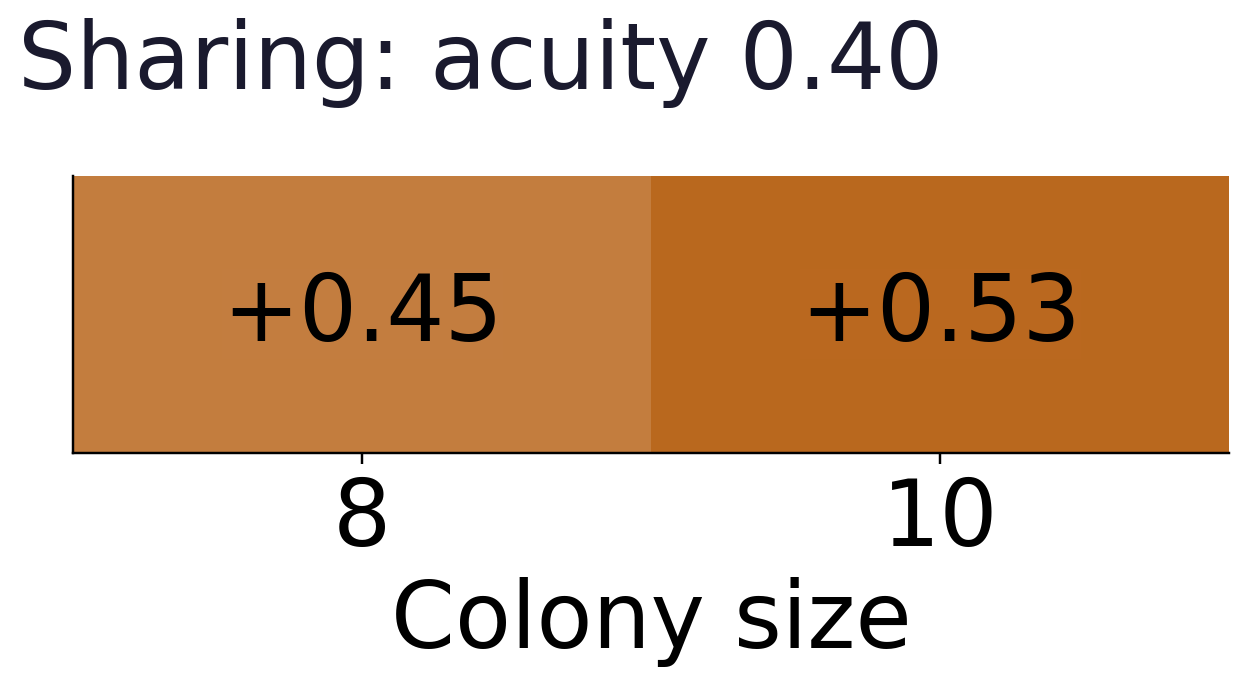
\includegraphics[keepaspectratio,width=0.98\linewidth,height=0.8\textheight,alt={Sharing, acuity 0.40: every signed accuracy gap in the displayed colony-size cells; common symmetric color scale and display-band hatch.}]{../figures/sensitivity_heatmap.slide-sharing-acuity-1-columns-4-5.png}
\refstepcounter{figure}\label{fig:sensitivity-heatmap-slide-panel-2}
\end{figure}
\end{frame}

\begin{frame}{Pattern 3: a conditional\ldots{} (part 8)}
\begin{figure}
\centering
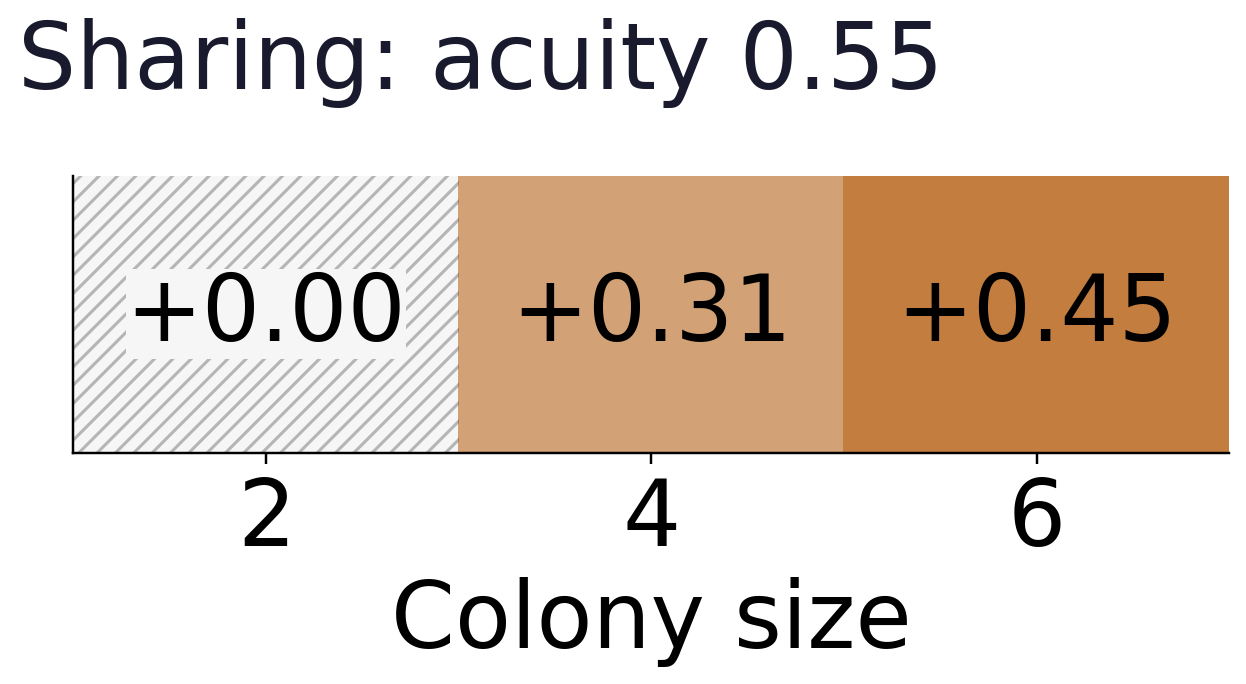
\includegraphics[keepaspectratio,width=0.98\linewidth,height=0.8\textheight,alt={Sharing, acuity 0.55: every signed accuracy gap in the displayed colony-size cells; common symmetric color scale and display-band hatch.}]{../figures/sensitivity_heatmap.slide-sharing-acuity-2-columns-1-3.png}
\refstepcounter{figure}\label{fig:sensitivity-heatmap-slide-panel-3}
\end{figure}
\end{frame}

\begin{frame}{Pattern 3: a conditional\ldots{} (part 9)}
\begin{figure}
\centering
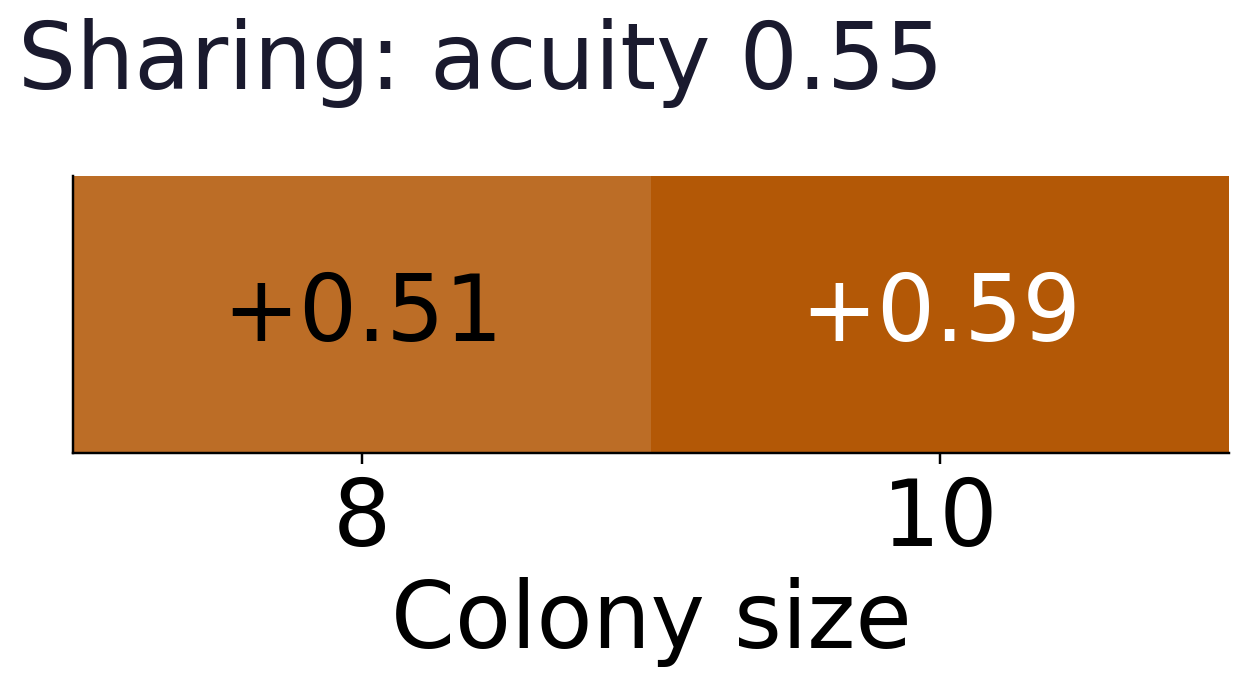
\includegraphics[keepaspectratio,width=0.98\linewidth,height=0.8\textheight,alt={Sharing, acuity 0.55: every signed accuracy gap in the displayed colony-size cells; common symmetric color scale and display-band hatch.}]{../figures/sensitivity_heatmap.slide-sharing-acuity-2-columns-4-5.png}
\refstepcounter{figure}\label{fig:sensitivity-heatmap-slide-panel-4}
\end{figure}
\end{frame}

\begin{frame}{Pattern 3: a conditional\ldots{} (part 10)}
\begin{figure}
\centering
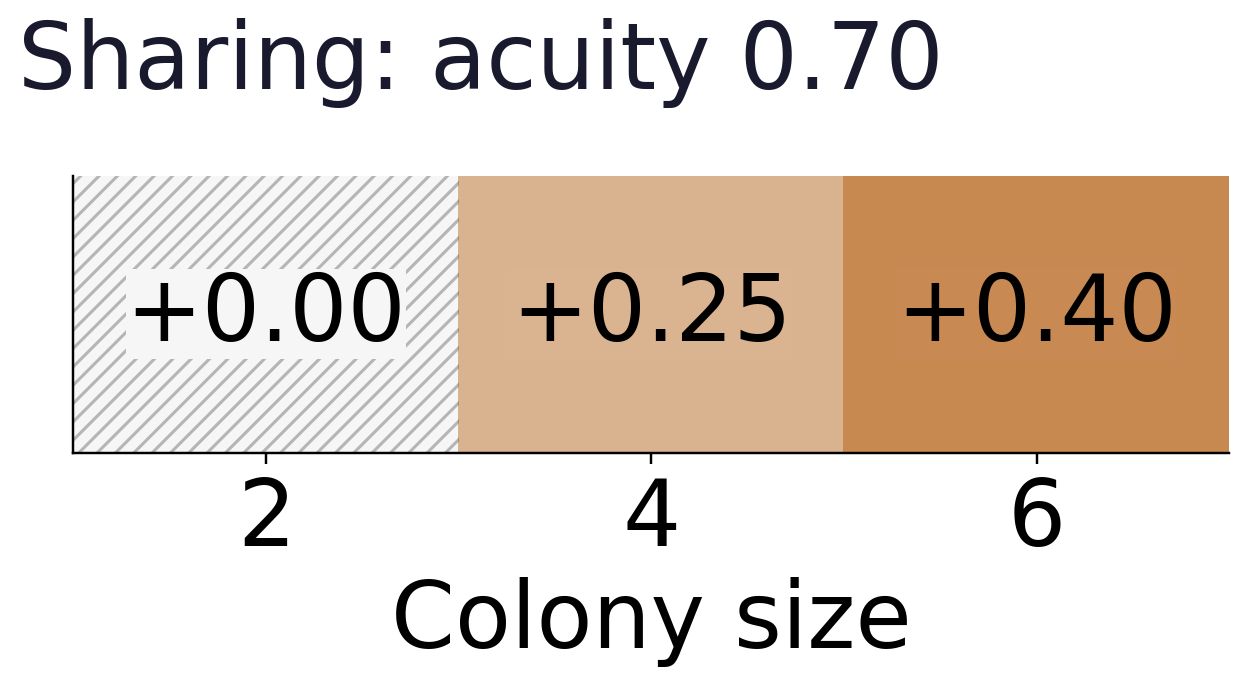
\includegraphics[keepaspectratio,width=0.98\linewidth,height=0.8\textheight,alt={Sharing, acuity 0.70: every signed accuracy gap in the displayed colony-size cells; common symmetric color scale and display-band hatch.}]{../figures/sensitivity_heatmap.slide-sharing-acuity-3-columns-1-3.png}
\refstepcounter{figure}\label{fig:sensitivity-heatmap-slide-panel-5}
\end{figure}
\end{frame}

\begin{frame}{Pattern 3: a conditional\ldots{} (part 11)}
\begin{figure}
\centering
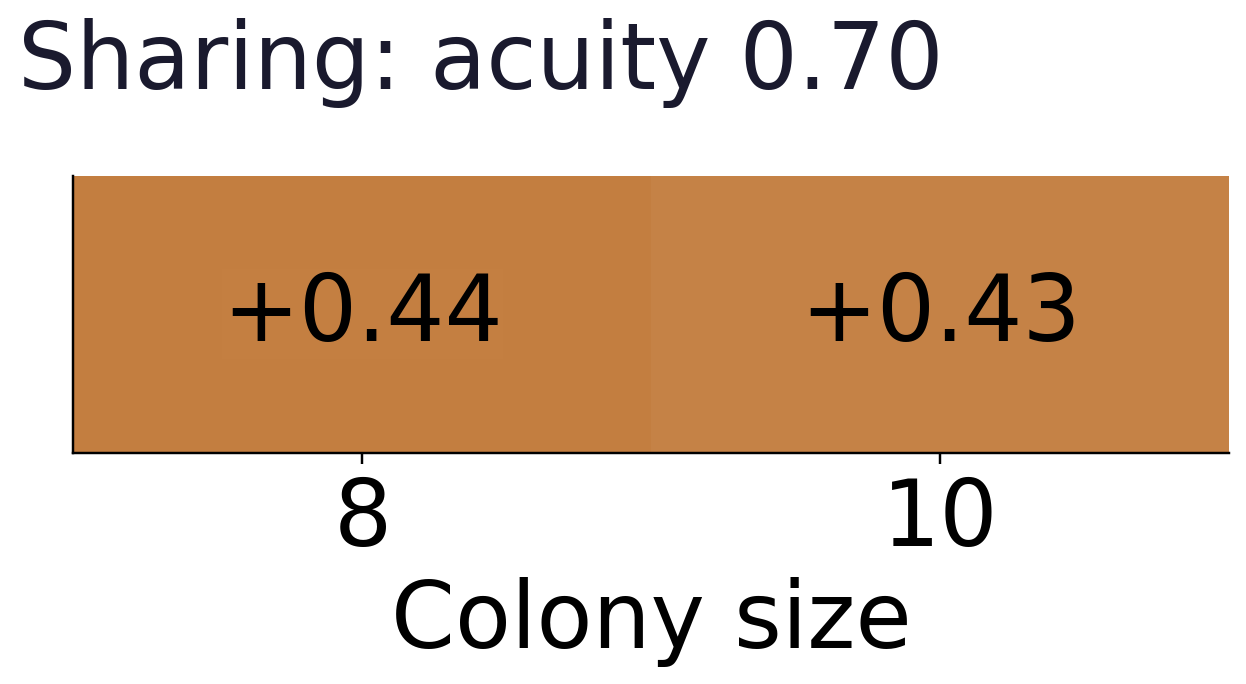
\includegraphics[keepaspectratio,width=0.98\linewidth,height=0.8\textheight,alt={Sharing, acuity 0.70: every signed accuracy gap in the displayed colony-size cells; common symmetric color scale and display-band hatch.}]{../figures/sensitivity_heatmap.slide-sharing-acuity-3-columns-4-5.png}
\refstepcounter{figure}\label{fig:sensitivity-heatmap-slide-panel-6}
\end{figure}
\end{frame}

\begin{frame}{Pattern 3: a conditional\ldots{} (part 12)}
\begin{figure}
\centering
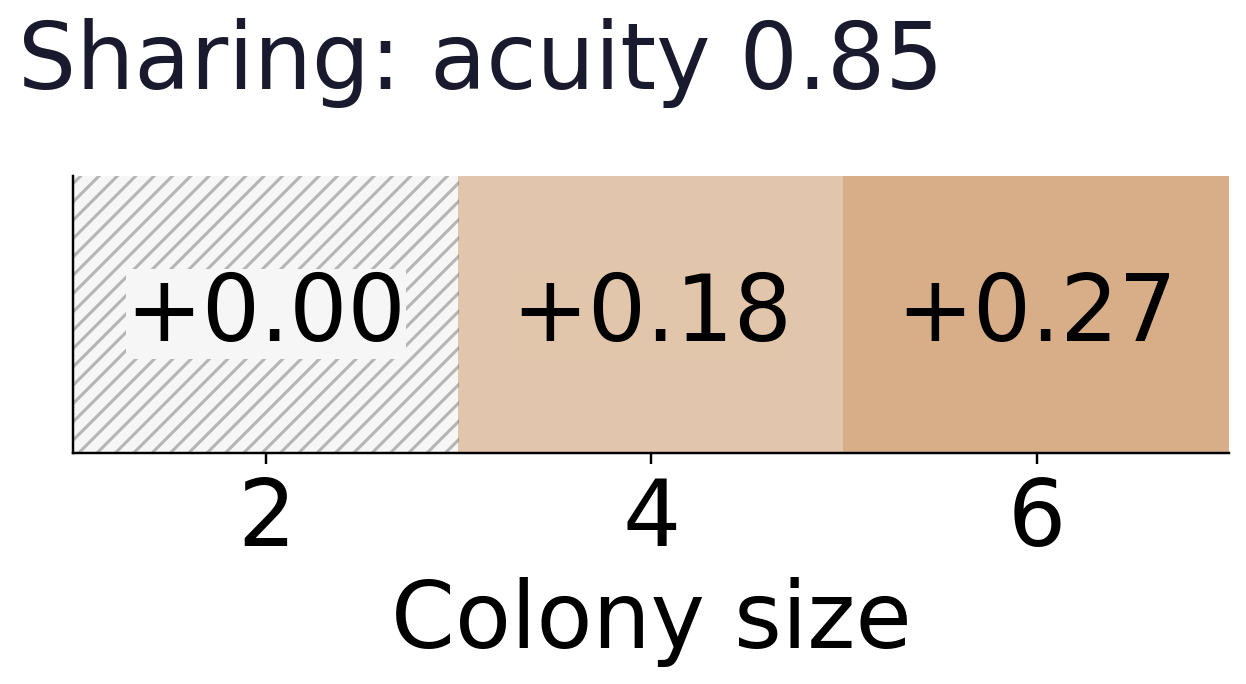
\includegraphics[keepaspectratio,width=0.98\linewidth,height=0.8\textheight,alt={Sharing, acuity 0.85: every signed accuracy gap in the displayed colony-size cells; common symmetric color scale and display-band hatch.}]{../figures/sensitivity_heatmap.slide-sharing-acuity-4-columns-1-3.png}
\refstepcounter{figure}\label{fig:sensitivity-heatmap-slide-panel-7}
\end{figure}
\end{frame}

\begin{frame}{Pattern 3: a conditional\ldots{} (part 13)}
\begin{figure}
\centering
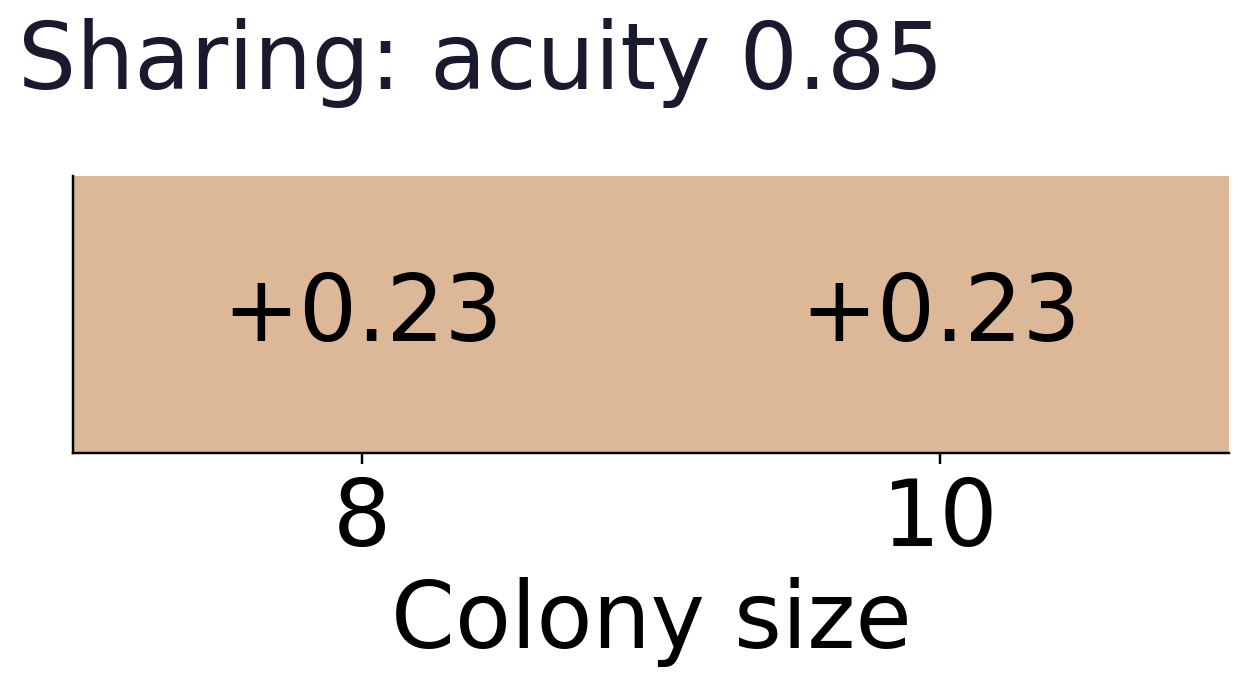
\includegraphics[keepaspectratio,width=0.98\linewidth,height=0.8\textheight,alt={Sharing, acuity 0.85: every signed accuracy gap in the displayed colony-size cells; common symmetric color scale and display-band hatch.}]{../figures/sensitivity_heatmap.slide-sharing-acuity-4-columns-4-5.png}
\refstepcounter{figure}\label{fig:sensitivity-heatmap-slide-panel-8}
\end{figure}
\end{frame}

\begin{frame}{Pattern 3: a conditional\ldots{} (part 14)}
\begin{figure}
\centering
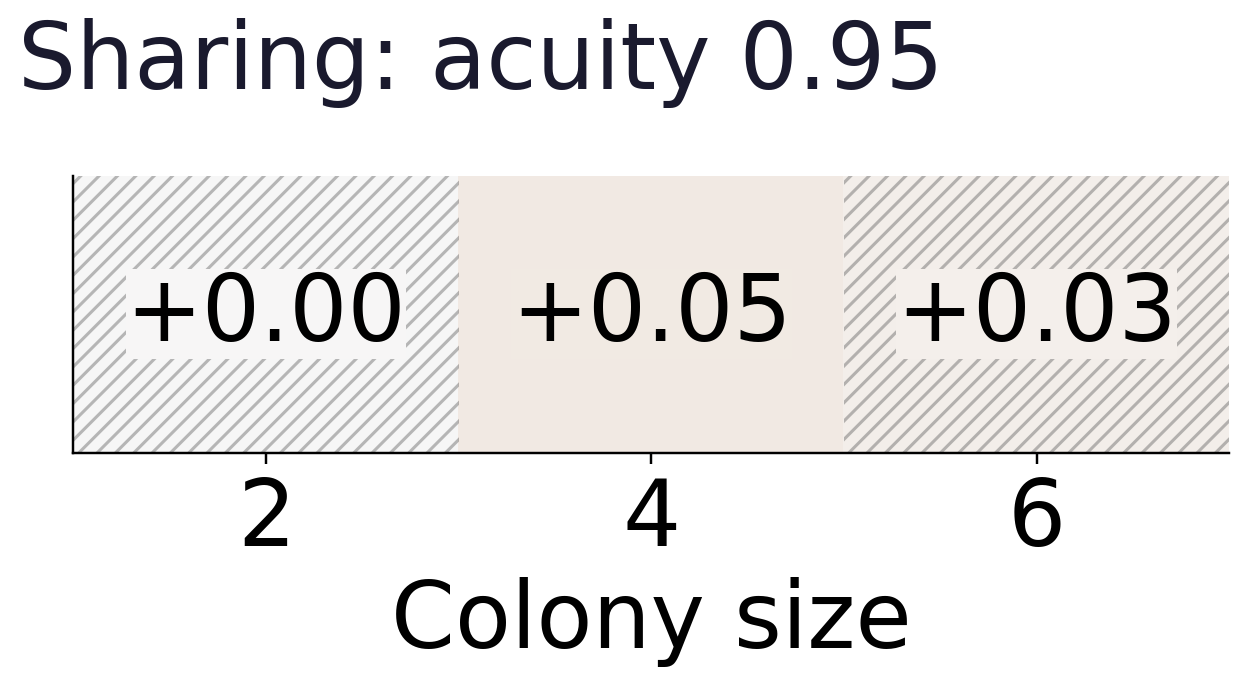
\includegraphics[keepaspectratio,width=0.98\linewidth,height=0.8\textheight,alt={Sharing, acuity 0.95: every signed accuracy gap in the displayed colony-size cells; common symmetric color scale and display-band hatch.}]{../figures/sensitivity_heatmap.slide-sharing-acuity-5-columns-1-3.png}
\refstepcounter{figure}\label{fig:sensitivity-heatmap-slide-panel-9}
\end{figure}
\end{frame}

\begin{frame}{Pattern 3: a conditional\ldots{} (part 15)}
\begin{figure}
\centering
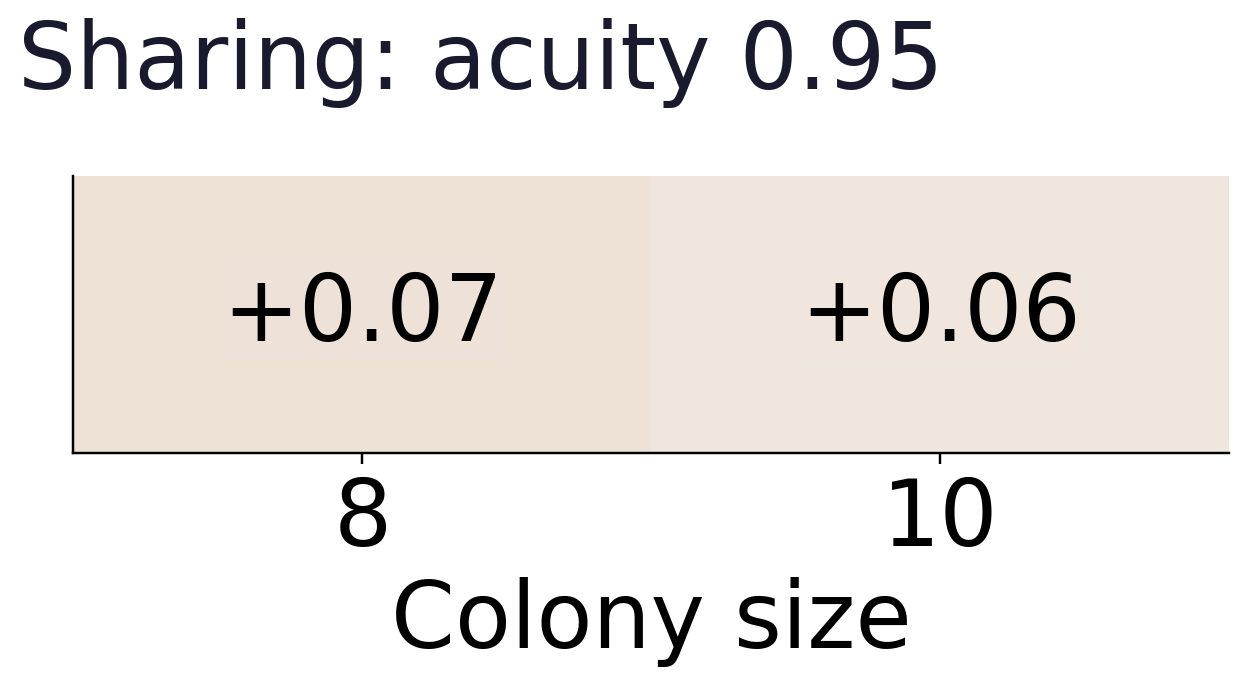
\includegraphics[keepaspectratio,width=0.98\linewidth,height=0.8\textheight,alt={Sharing, acuity 0.95: every signed accuracy gap in the displayed colony-size cells; common symmetric color scale and display-band hatch.}]{../figures/sensitivity_heatmap.slide-sharing-acuity-5-columns-4-5.png}
\refstepcounter{figure}\label{fig:sensitivity-heatmap-slide-panel-10}
\end{figure}
\end{frame}

\begin{frame}{Pattern 3: a conditional\ldots{} (part 16)}
\begin{figure}
\centering
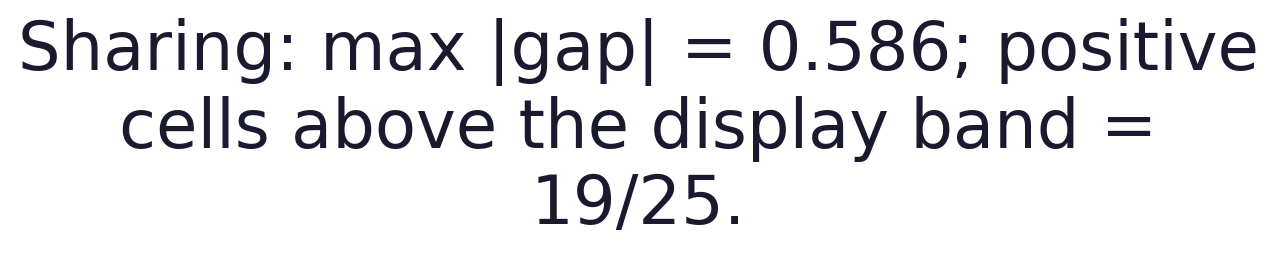
\includegraphics[keepaspectratio,width=0.98\linewidth,height=0.8\textheight,alt={Sharing: max \textbar gap\textbar{} = 0.586; positive cells above the display band = 19/25.}]{../figures/sensitivity_heatmap.slide-sharing-summary.png}
\refstepcounter{figure}\label{fig:sensitivity-heatmap-slide-panel-11}
\end{figure}
\end{frame}

\begin{frame}{Pattern 3: a conditional\ldots{} (part 17)}
\begin{figure}
\centering
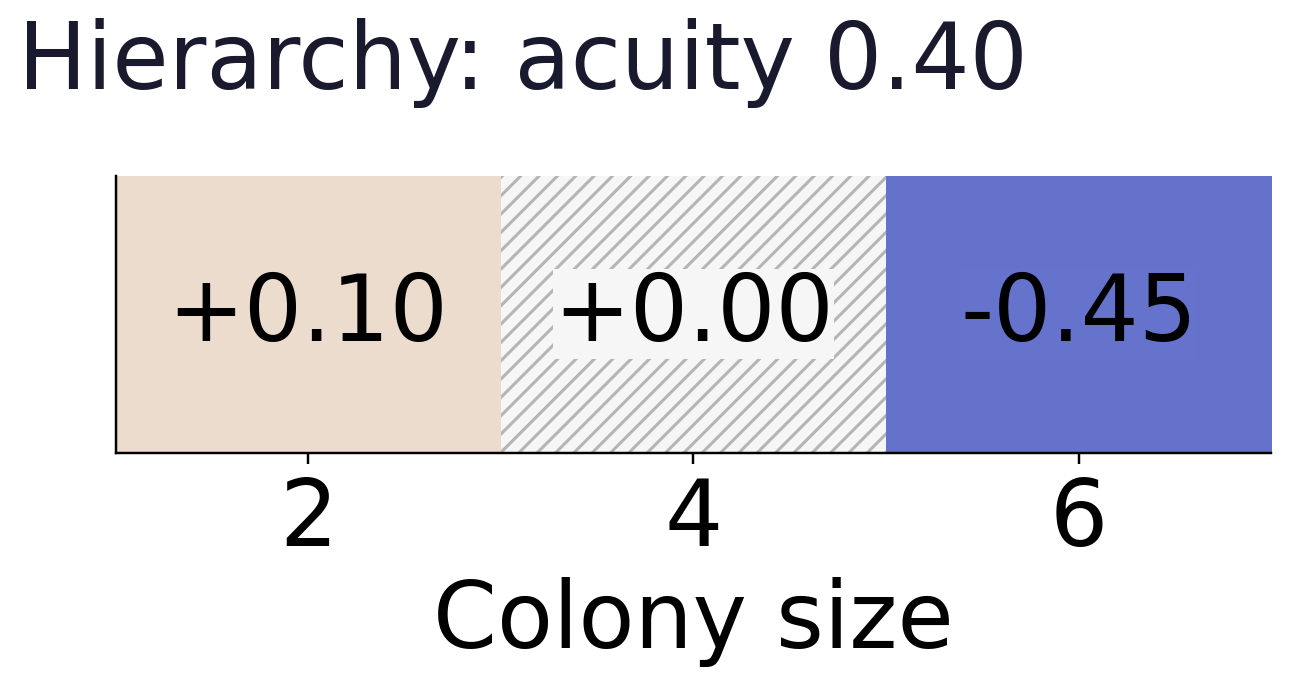
\includegraphics[keepaspectratio,width=0.98\linewidth,height=0.8\textheight,alt={Hierarchy, acuity 0.40: every signed accuracy gap in the displayed colony-size cells; common symmetric color scale and display-band hatch.}]{../figures/sensitivity_heatmap.slide-hierarchy-acuity-1-columns-1-3.png}
\refstepcounter{figure}\label{fig:sensitivity-heatmap-slide-panel-12}
\end{figure}
\end{frame}

\begin{frame}{Pattern 3: a conditional\ldots{} (part 18)}
\begin{figure}
\centering
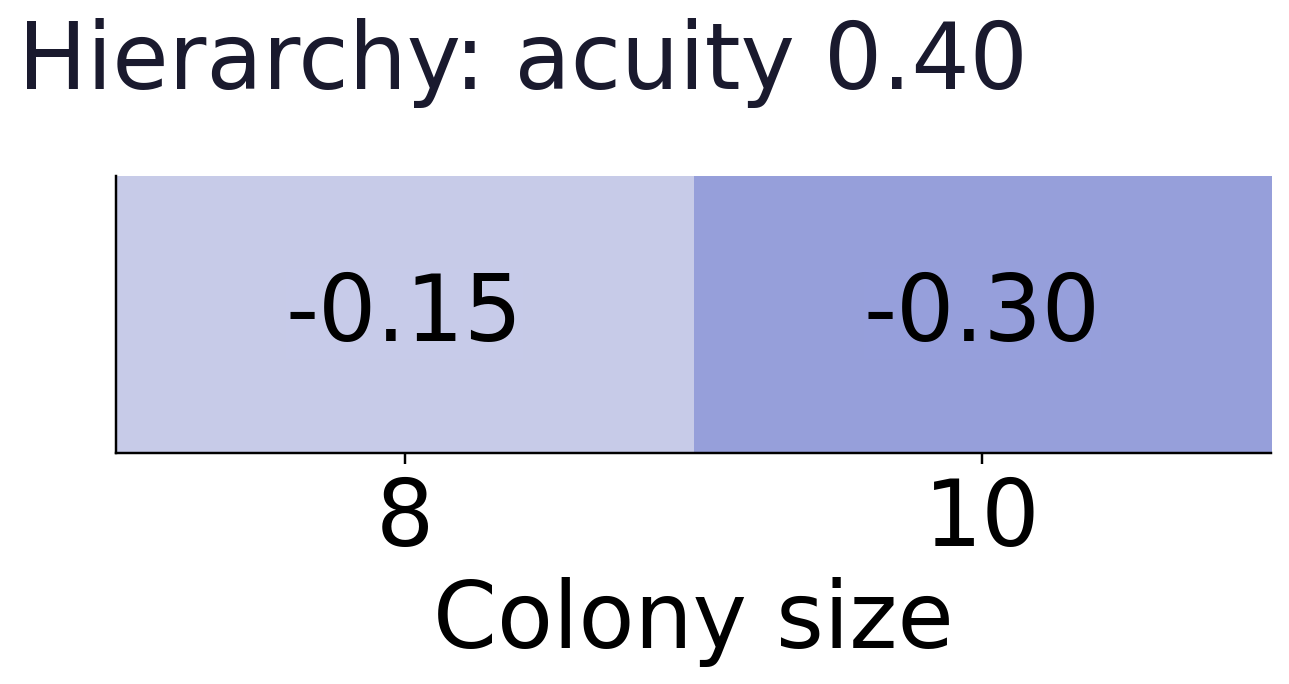
\includegraphics[keepaspectratio,width=0.98\linewidth,height=0.8\textheight,alt={Hierarchy, acuity 0.40: every signed accuracy gap in the displayed colony-size cells; common symmetric color scale and display-band hatch.}]{../figures/sensitivity_heatmap.slide-hierarchy-acuity-1-columns-4-5.png}
\refstepcounter{figure}\label{fig:sensitivity-heatmap-slide-panel-13}
\end{figure}
\end{frame}

\begin{frame}{Pattern 3: a conditional\ldots{} (part 19)}
\begin{figure}
\centering
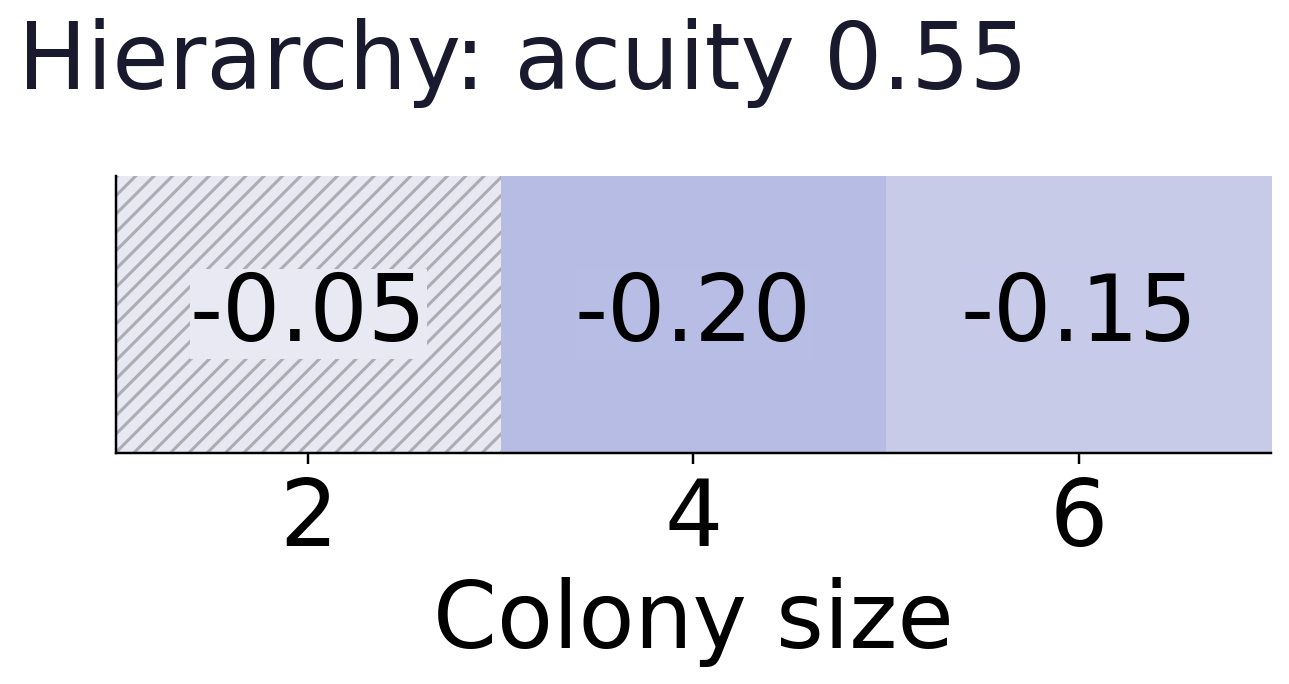
\includegraphics[keepaspectratio,width=0.98\linewidth,height=0.8\textheight,alt={Hierarchy, acuity 0.55: every signed accuracy gap in the displayed colony-size cells; common symmetric color scale and display-band hatch.}]{../figures/sensitivity_heatmap.slide-hierarchy-acuity-2-columns-1-3.png}
\refstepcounter{figure}\label{fig:sensitivity-heatmap-slide-panel-14}
\end{figure}
\end{frame}

\begin{frame}{Pattern 3: a conditional\ldots{} (part 20)}
\begin{figure}
\centering
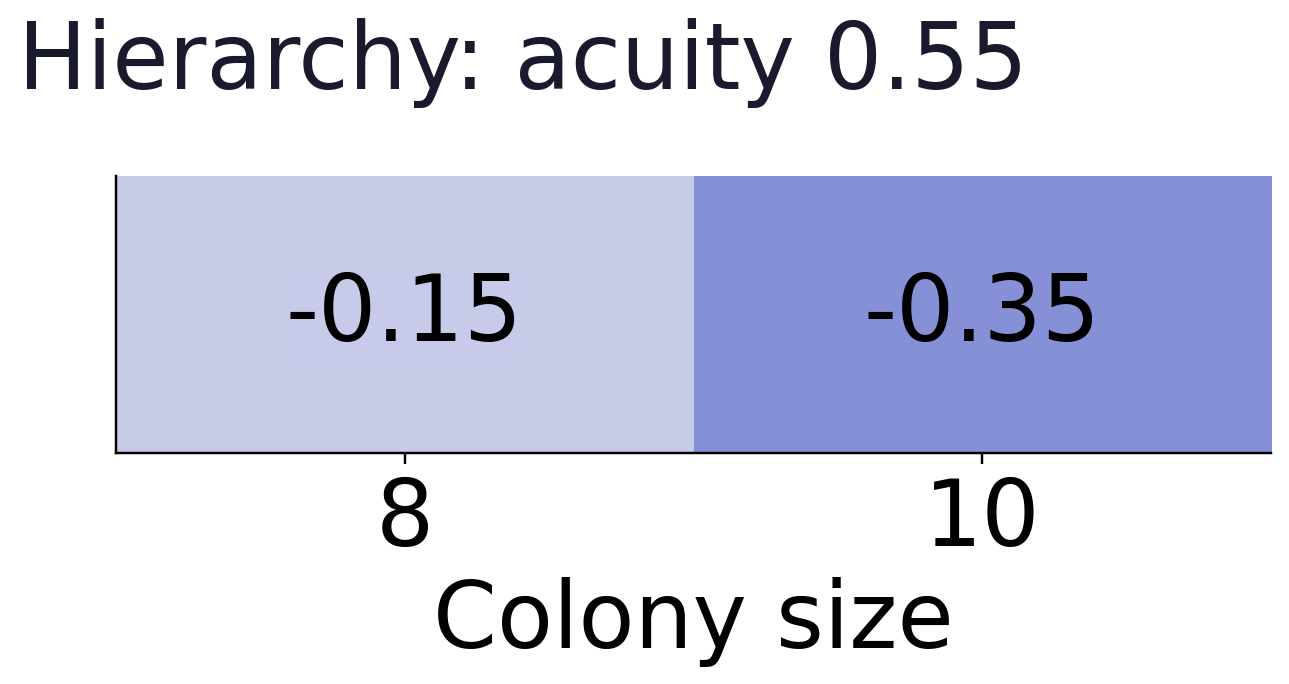
\includegraphics[keepaspectratio,width=0.98\linewidth,height=0.8\textheight,alt={Hierarchy, acuity 0.55: every signed accuracy gap in the displayed colony-size cells; common symmetric color scale and display-band hatch.}]{../figures/sensitivity_heatmap.slide-hierarchy-acuity-2-columns-4-5.png}
\refstepcounter{figure}\label{fig:sensitivity-heatmap-slide-panel-15}
\end{figure}
\end{frame}

\begin{frame}{Pattern 3: a conditional\ldots{} (part 21)}
\begin{figure}
\centering
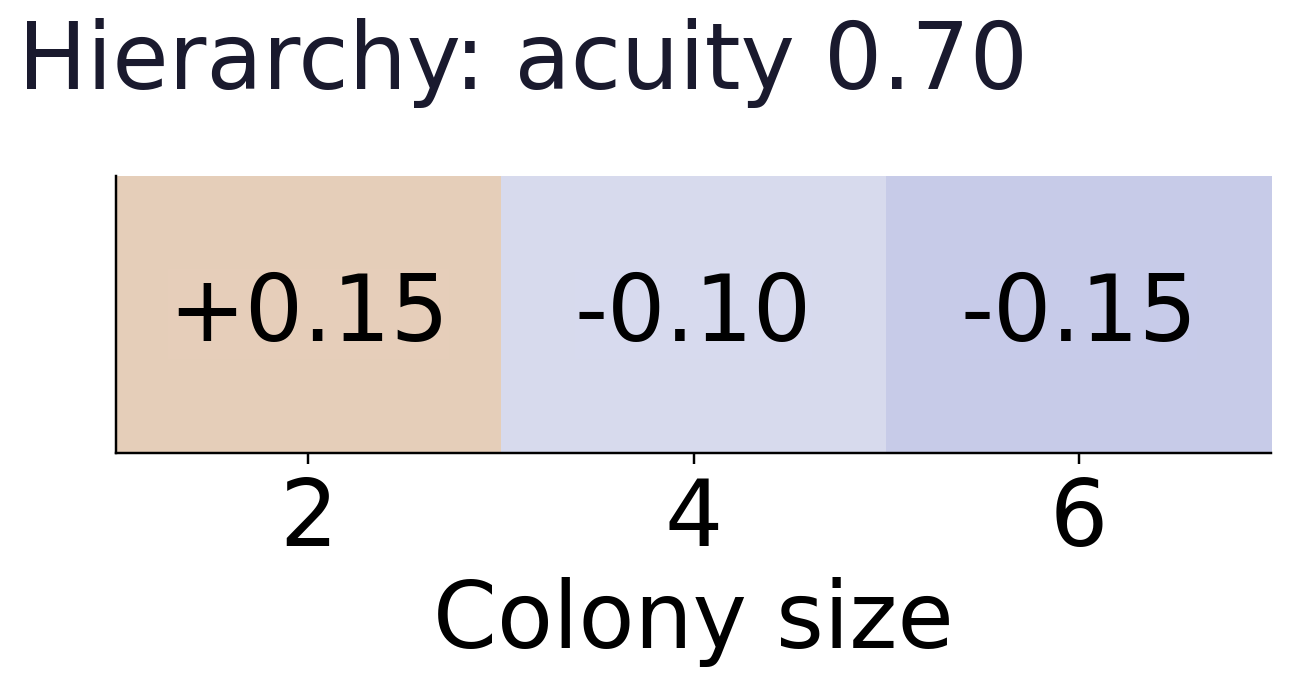
\includegraphics[keepaspectratio,width=0.98\linewidth,height=0.8\textheight,alt={Hierarchy, acuity 0.70: every signed accuracy gap in the displayed colony-size cells; common symmetric color scale and display-band hatch.}]{../figures/sensitivity_heatmap.slide-hierarchy-acuity-3-columns-1-3.png}
\refstepcounter{figure}\label{fig:sensitivity-heatmap-slide-panel-16}
\end{figure}
\end{frame}

\begin{frame}{Pattern 3: a conditional\ldots{} (part 22)}
\begin{figure}
\centering
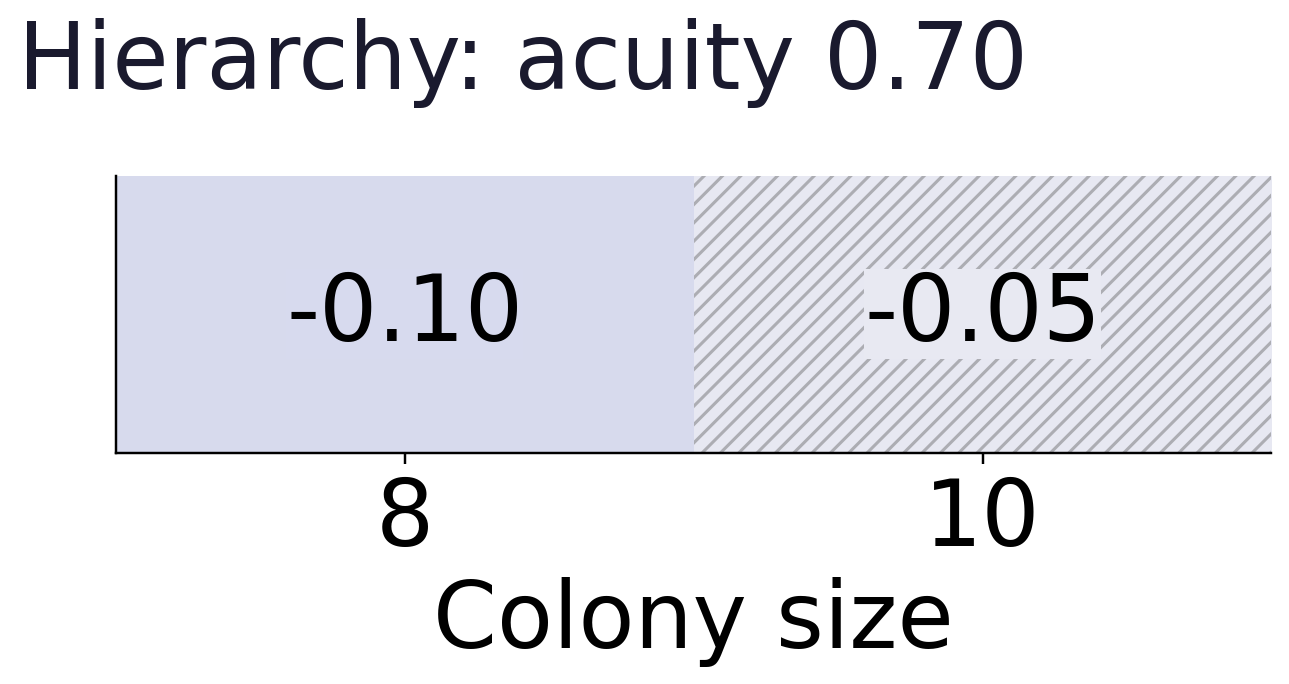
\includegraphics[keepaspectratio,width=0.98\linewidth,height=0.8\textheight,alt={Hierarchy, acuity 0.70: every signed accuracy gap in the displayed colony-size cells; common symmetric color scale and display-band hatch.}]{../figures/sensitivity_heatmap.slide-hierarchy-acuity-3-columns-4-5.png}
\refstepcounter{figure}\label{fig:sensitivity-heatmap-slide-panel-17}
\end{figure}
\end{frame}

\begin{frame}{Pattern 3: a conditional\ldots{} (part 23)}
\begin{figure}
\centering
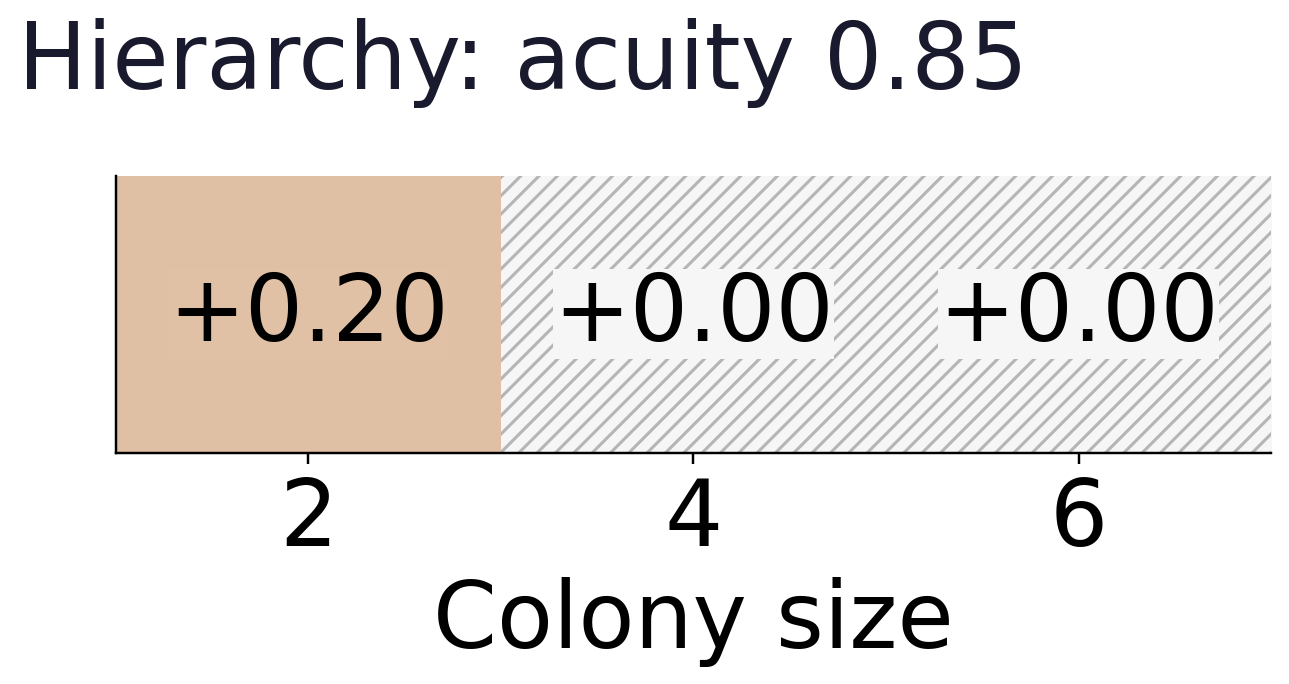
\includegraphics[keepaspectratio,width=0.98\linewidth,height=0.8\textheight,alt={Hierarchy, acuity 0.85: every signed accuracy gap in the displayed colony-size cells; common symmetric color scale and display-band hatch.}]{../figures/sensitivity_heatmap.slide-hierarchy-acuity-4-columns-1-3.png}
\refstepcounter{figure}\label{fig:sensitivity-heatmap-slide-panel-18}
\end{figure}
\end{frame}

\begin{frame}{Pattern 3: a conditional\ldots{} (part 24)}
\begin{figure}
\centering
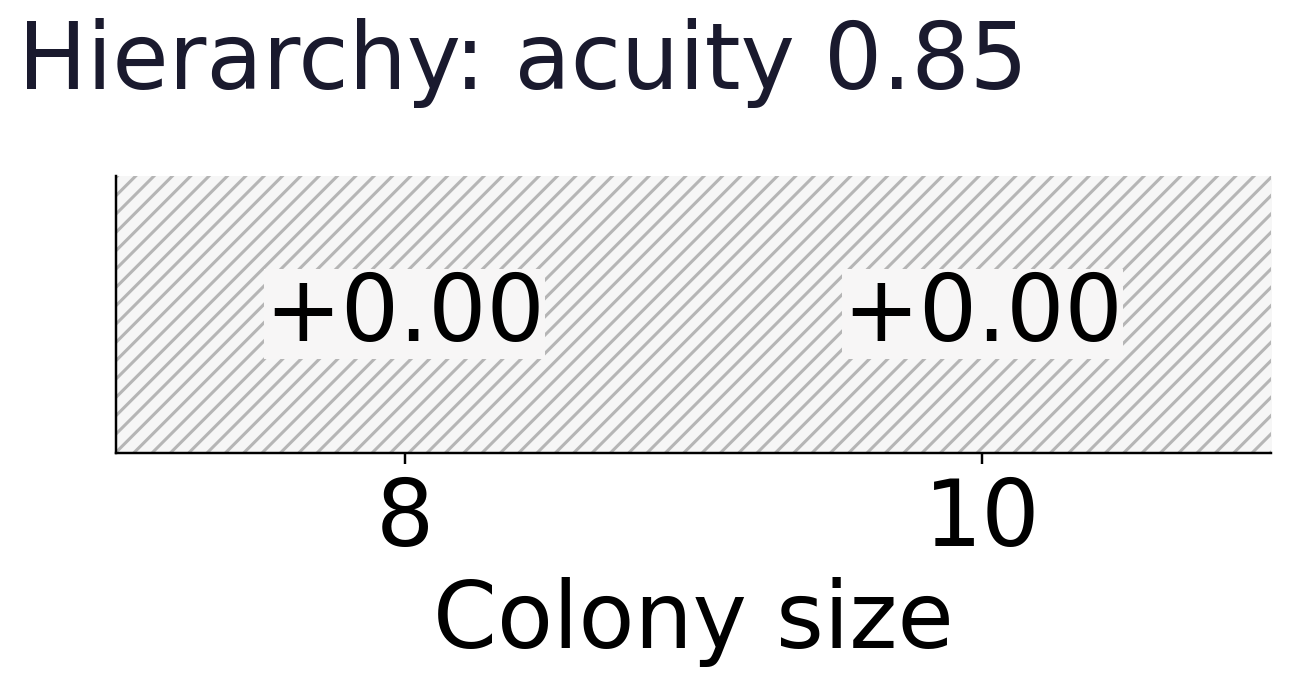
\includegraphics[keepaspectratio,width=0.98\linewidth,height=0.8\textheight,alt={Hierarchy, acuity 0.85: every signed accuracy gap in the displayed colony-size cells; common symmetric color scale and display-band hatch.}]{../figures/sensitivity_heatmap.slide-hierarchy-acuity-4-columns-4-5.png}
\refstepcounter{figure}\label{fig:sensitivity-heatmap-slide-panel-19}
\end{figure}
\end{frame}

\begin{frame}{Pattern 3: a conditional\ldots{} (part 25)}
\begin{figure}
\centering
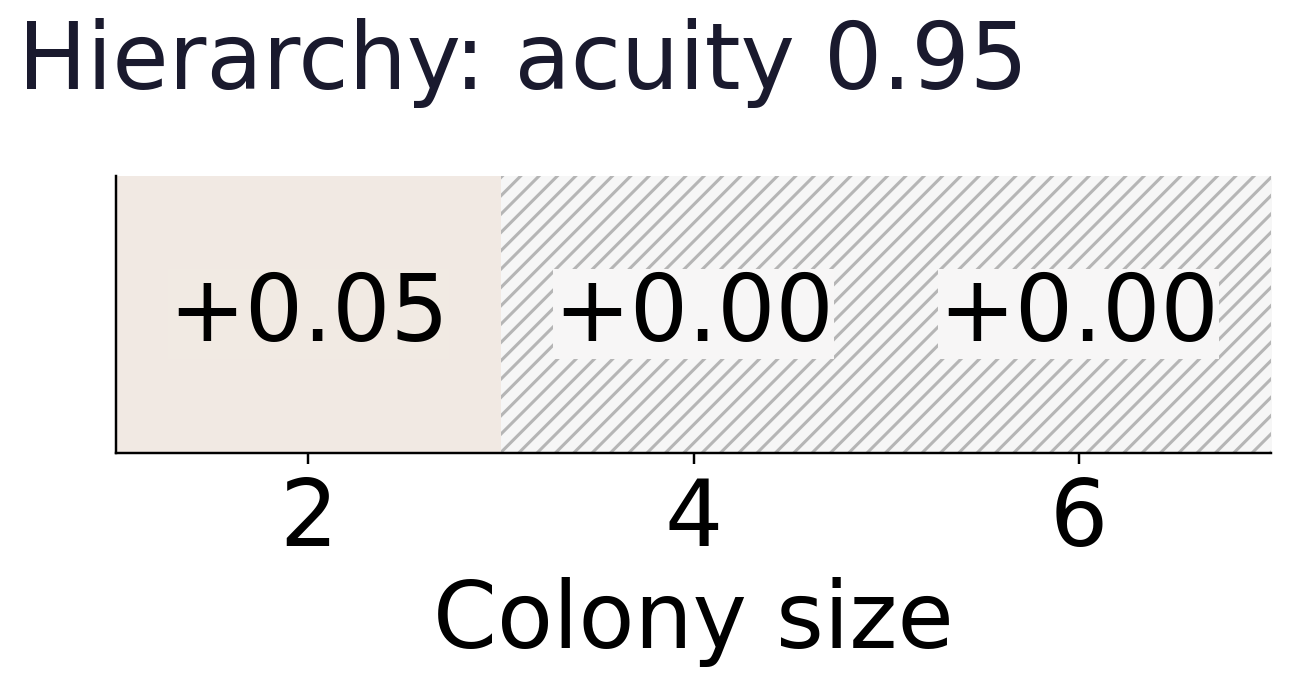
\includegraphics[keepaspectratio,width=0.98\linewidth,height=0.8\textheight,alt={Hierarchy, acuity 0.95: every signed accuracy gap in the displayed colony-size cells; common symmetric color scale and display-band hatch.}]{../figures/sensitivity_heatmap.slide-hierarchy-acuity-5-columns-1-3.png}
\refstepcounter{figure}\label{fig:sensitivity-heatmap-slide-panel-20}
\end{figure}
\end{frame}

\begin{frame}{Pattern 3: a conditional\ldots{} (part 26)}
\begin{figure}
\centering
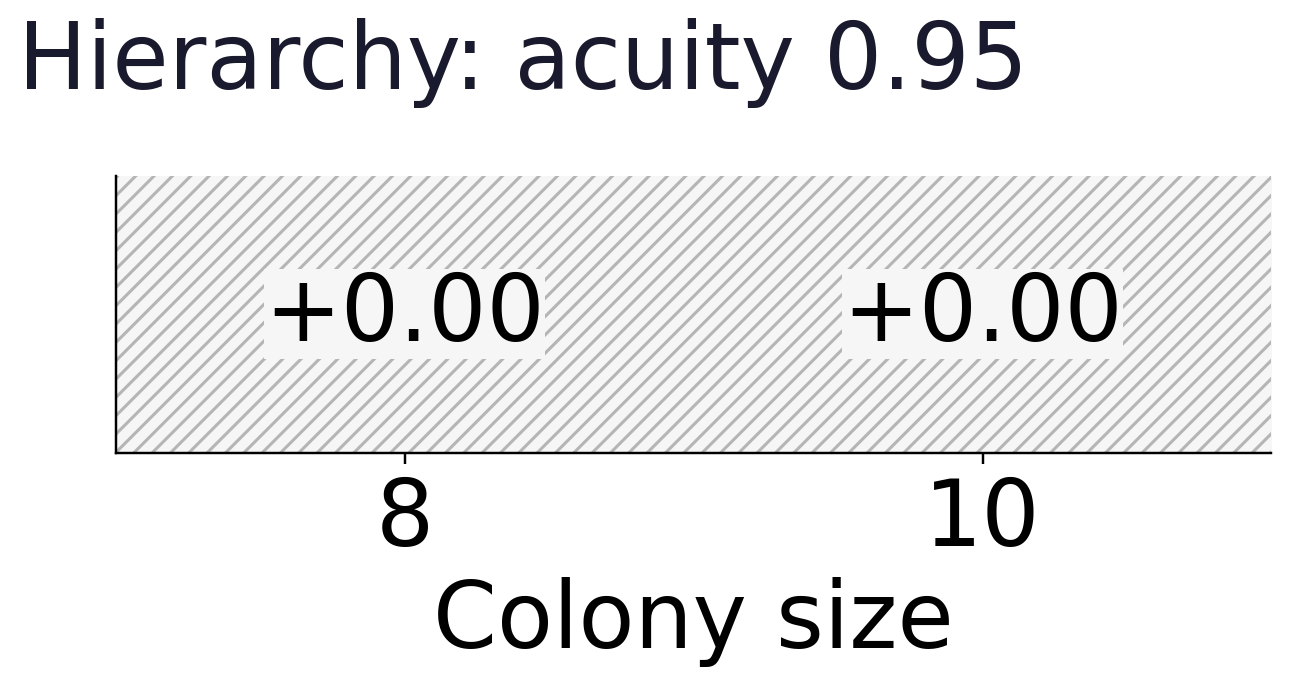
\includegraphics[keepaspectratio,width=0.98\linewidth,height=0.8\textheight,alt={Hierarchy, acuity 0.95: every signed accuracy gap in the displayed colony-size cells; common symmetric color scale and display-band hatch.}]{../figures/sensitivity_heatmap.slide-hierarchy-acuity-5-columns-4-5.png}
\refstepcounter{figure}\label{fig:sensitivity-heatmap-slide-panel-21}
\end{figure}
\end{frame}

\begin{frame}{Pattern 3: a conditional\ldots{} (part 27)}
\begin{figure}
\centering
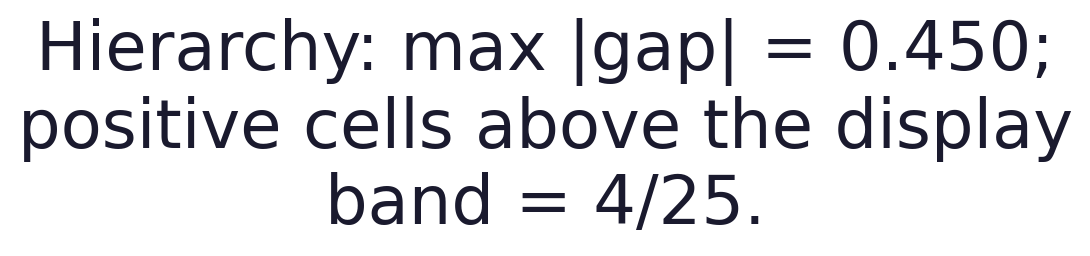
\includegraphics[keepaspectratio,width=0.98\linewidth,height=0.8\textheight,alt={Hierarchy: max \textbar gap\textbar{} = 0.450; positive cells above the display band = 4/25.}]{../figures/sensitivity_heatmap.slide-hierarchy-summary.png}
\refstepcounter{figure}\label{fig:sensitivity-heatmap-slide-panel-22}
\end{figure}
\end{frame}

\begin{frame}{Pattern 3: a conditional\ldots{} (part 28)}
\begin{figure}
\centering
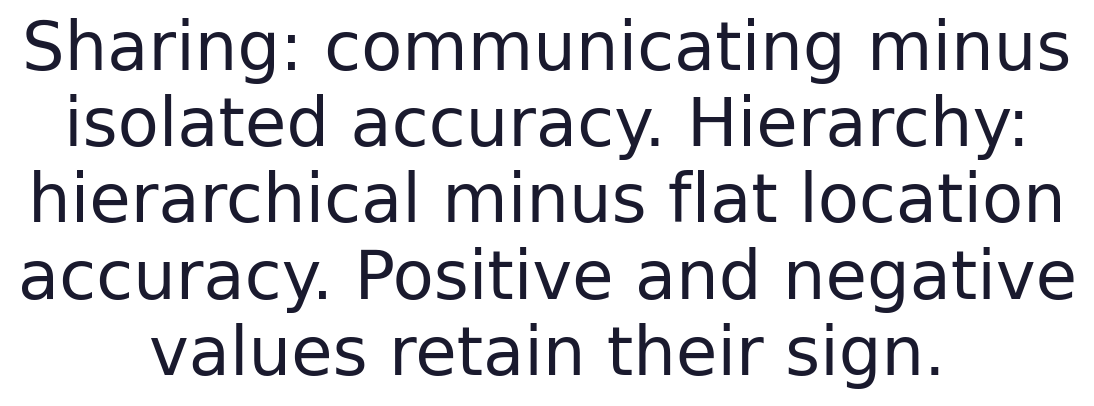
\includegraphics[keepaspectratio,width=0.98\linewidth,height=0.8\textheight,alt={Sharing: communicating minus isolated accuracy. Hierarchy: hierarchical minus flat location accuracy. Positive and negative values retain their sign.}]{../figures/sensitivity_heatmap.slide-direction.png}
\refstepcounter{figure}\label{fig:sensitivity-heatmap-slide-panel-23}
\end{figure}
\end{frame}

\begin{frame}{Pattern 3: a conditional\ldots{} (part 29)}
\begin{figure}
\centering
\includegraphics[keepaspectratio,width=0.98\linewidth,height=0.8\textheight,alt={Common signed color scale: {[}-0.5861, 0.5861{]}. Every cell prints its value; panels keep original acuity and colony ordering.}]{../figures/sensitivity_heatmap.slide-scale.png}
\refstepcounter{figure}\label{fig:sensitivity-heatmap-slide-panel-24}
\end{figure}
\end{frame}

\begin{frame}{Pattern 3: a conditional\ldots{} (part 30)}
\begin{figure}
\centering
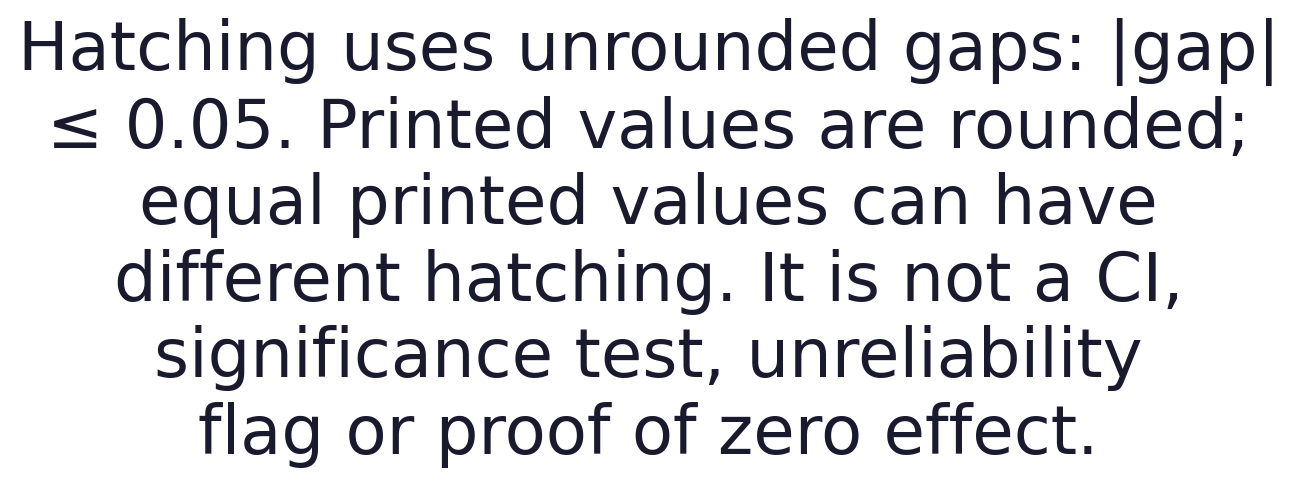
\includegraphics[keepaspectratio,width=0.98\linewidth,height=0.8\textheight,alt={Hatching uses unrounded gaps: \textbar gap\textbar{} ≤ 0.05. Printed values are rounded; equal printed values can have different hatching. It is not a CI, significance test, unreliability flag or proof of zero effect.}]{../figures/sensitivity_heatmap.slide-hatching.png}
\refstepcounter{figure}\label{fig:sensitivity-heatmap-slide-panel-25}
\end{figure}
\end{frame}

\begin{frame}{Pattern 3: a conditional\ldots{} (part 31)}
\begin{figure}
\centering
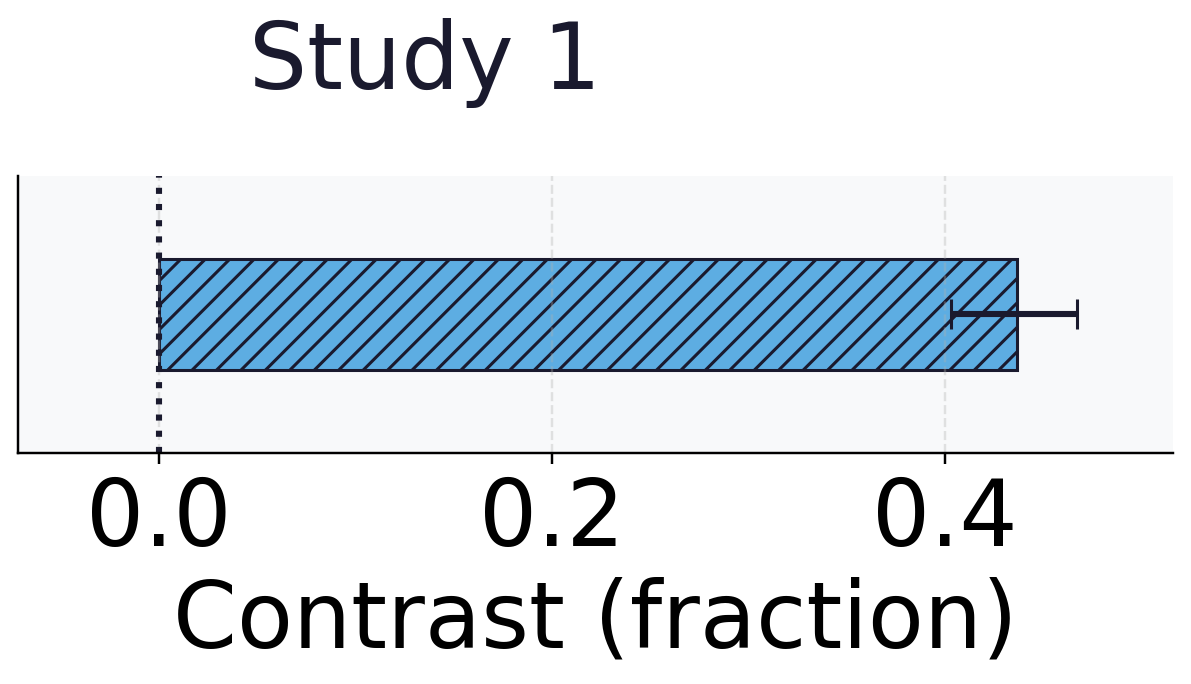
\includegraphics[keepaspectratio,width=0.98\linewidth,height=0.8\textheight,alt={Study 1
Belief sharing: mean and seed-bootstrap interval on the shared fraction facet scale.}]{../figures/cross_study_summary.slide-fraction-study-1.png}
\refstepcounter{figure}\label{fig:cross-study-summary-slide-panel-1}
\end{figure}
\end{frame}

\begin{frame}{Pattern 3: a conditional\ldots{} (part 32)}
\begin{figure}
\centering
\includegraphics[keepaspectratio,width=0.98\linewidth,height=0.8\textheight,alt={Study 1 Belief sharing. Mean +0.437; 95\% interval {[}+0.4034, +0.4675{]} fraction.}]{../figures/cross_study_summary.slide-fraction-study-1-values.png}
\refstepcounter{figure}\label{fig:cross-study-summary-slide-panel-2}
\end{figure}
\end{frame}

\begin{frame}{Pattern 3: a conditional\ldots{} (part 33)}
\begin{figure}
\centering
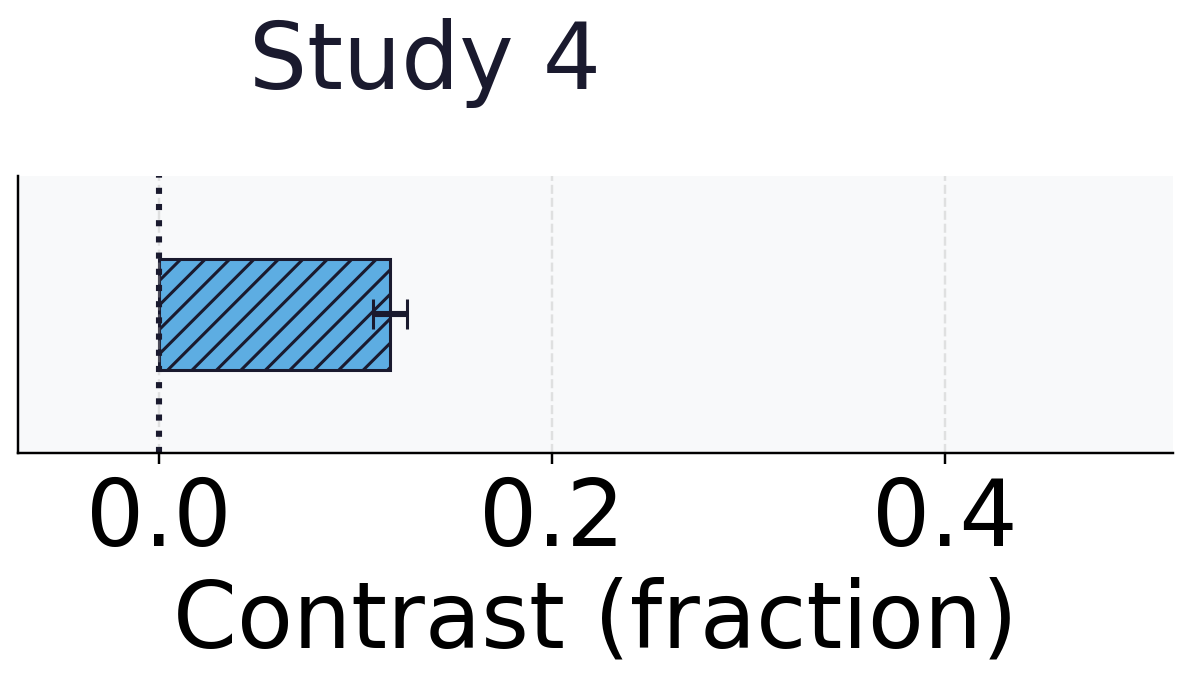
\includegraphics[keepaspectratio,width=0.98\linewidth,height=0.8\textheight,alt={Study 4
Within-run
display-selected maximum: mean and seed-bootstrap interval on the shared fraction facet scale.}]{../figures/cross_study_summary.slide-fraction-study-2.png}
\refstepcounter{figure}\label{fig:cross-study-summary-slide-panel-3}
\end{figure}
\end{frame}

\begin{frame}{Pattern 3: a conditional\ldots{} (part 34)}
\begin{figure}
\centering
\includegraphics[keepaspectratio,width=0.98\linewidth,height=0.8\textheight,alt={Study 4 Within-run display-selected maximum. Mean +0.1175; 95\% interval {[}+0.109, +0.1262{]} fraction.}]{../figures/cross_study_summary.slide-fraction-study-2-values.png}
\refstepcounter{figure}\label{fig:cross-study-summary-slide-panel-4}
\end{figure}
\end{frame}

\begin{frame}{Pattern 3: a conditional\ldots{} (part 35)}
\begin{figure}
\centering
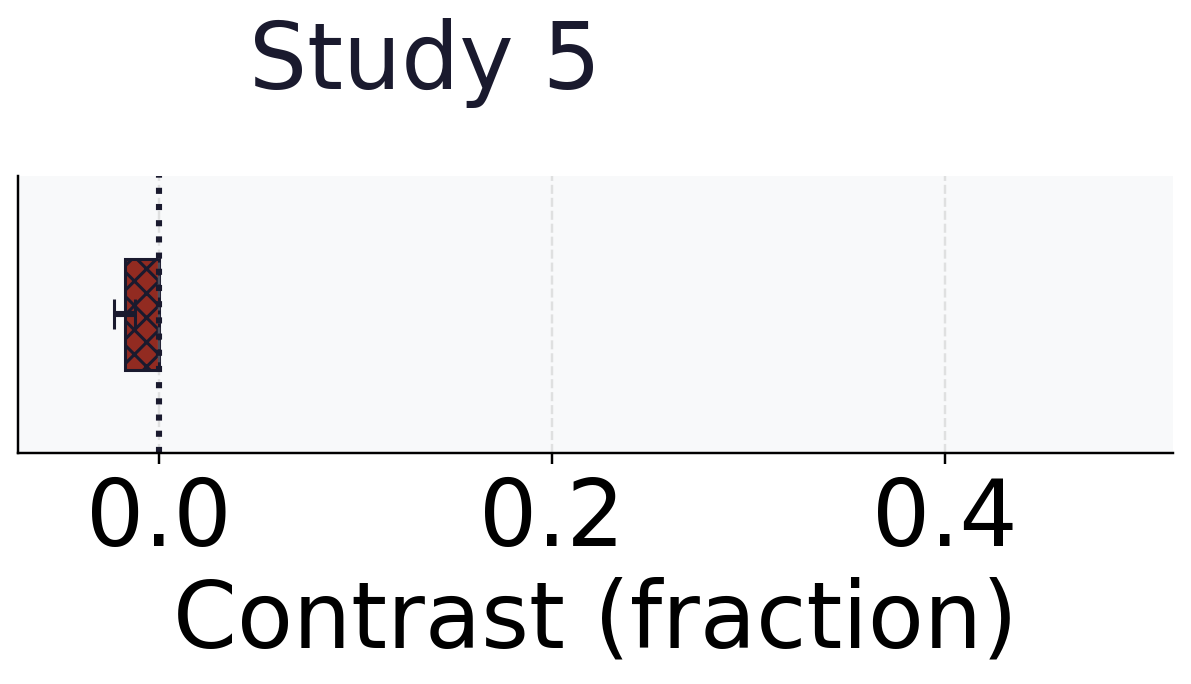
\includegraphics[keepaspectratio,width=0.98\linewidth,height=0.8\textheight,alt={Study 5
Moving world (EFE): mean and seed-bootstrap interval on the shared fraction facet scale.}]{../figures/cross_study_summary.slide-fraction-study-3.png}
\refstepcounter{figure}\label{fig:cross-study-summary-slide-panel-5}
\end{figure}
\end{frame}

\begin{frame}{Pattern 3: a conditional\ldots{} (part 36)}
\begin{figure}
\centering
\includegraphics[keepaspectratio,width=0.98\linewidth,height=0.8\textheight,alt={Study 5 Moving world (EFE). Mean -0.01758; 95\% interval {[}-0.02305, -0.0125{]} fraction.}]{../figures/cross_study_summary.slide-fraction-study-3-values.png}
\refstepcounter{figure}\label{fig:cross-study-summary-slide-panel-6}
\end{figure}
\end{frame}

\begin{frame}{Pattern 3: a conditional\ldots{} (part 37)}
\begin{figure}
\centering
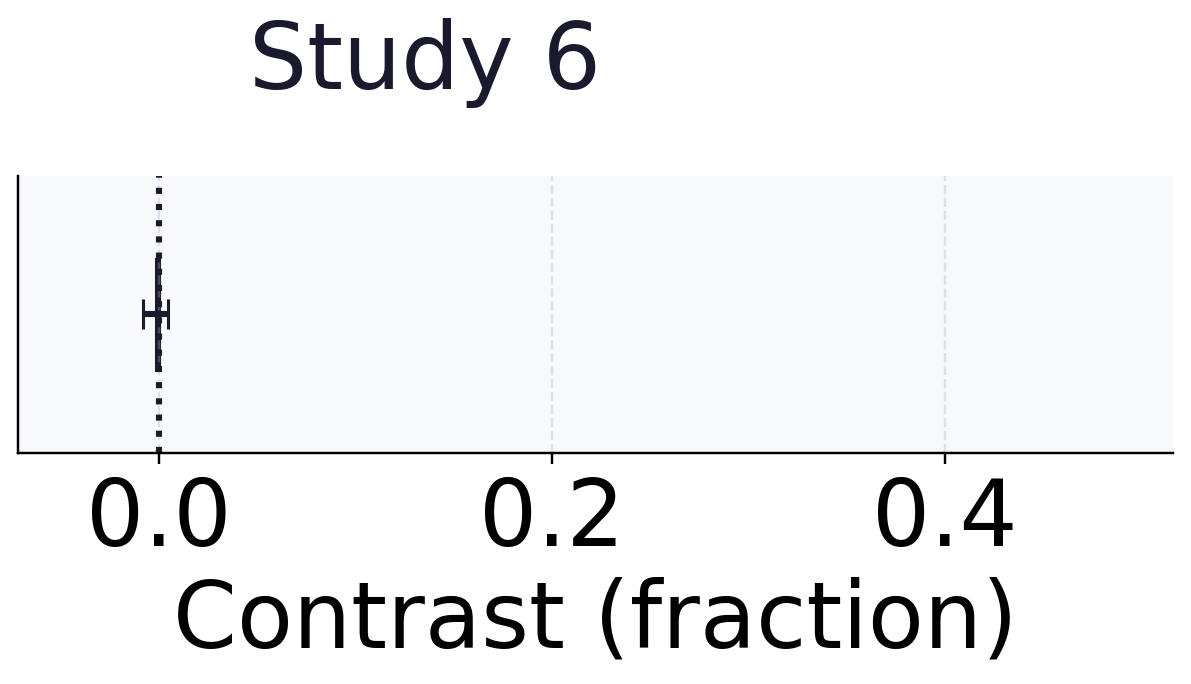
\includegraphics[keepaspectratio,width=0.98\linewidth,height=0.8\textheight,alt={Study 6
2-level hierarchical POMDP: mean and seed-bootstrap interval on the shared fraction facet scale.}]{../figures/cross_study_summary.slide-fraction-study-4.png}
\refstepcounter{figure}\label{fig:cross-study-summary-slide-panel-7}
\end{figure}
\end{frame}

\begin{frame}{Pattern 3: a conditional\ldots{} (part 38)}
\begin{figure}
\centering
\includegraphics[keepaspectratio,width=0.98\linewidth,height=0.8\textheight,alt={Study 6 2-level hierarchical POMDP. Mean -0.001563; 95\% interval {[}-0.008203, +0.004687{]} fraction.}]{../figures/cross_study_summary.slide-fraction-study-4-values.png}
\refstepcounter{figure}\label{fig:cross-study-summary-slide-panel-8}
\end{figure}
\end{frame}

\begin{frame}{Pattern 3: a conditional\ldots{} (part 39)}
\begin{figure}
\centering
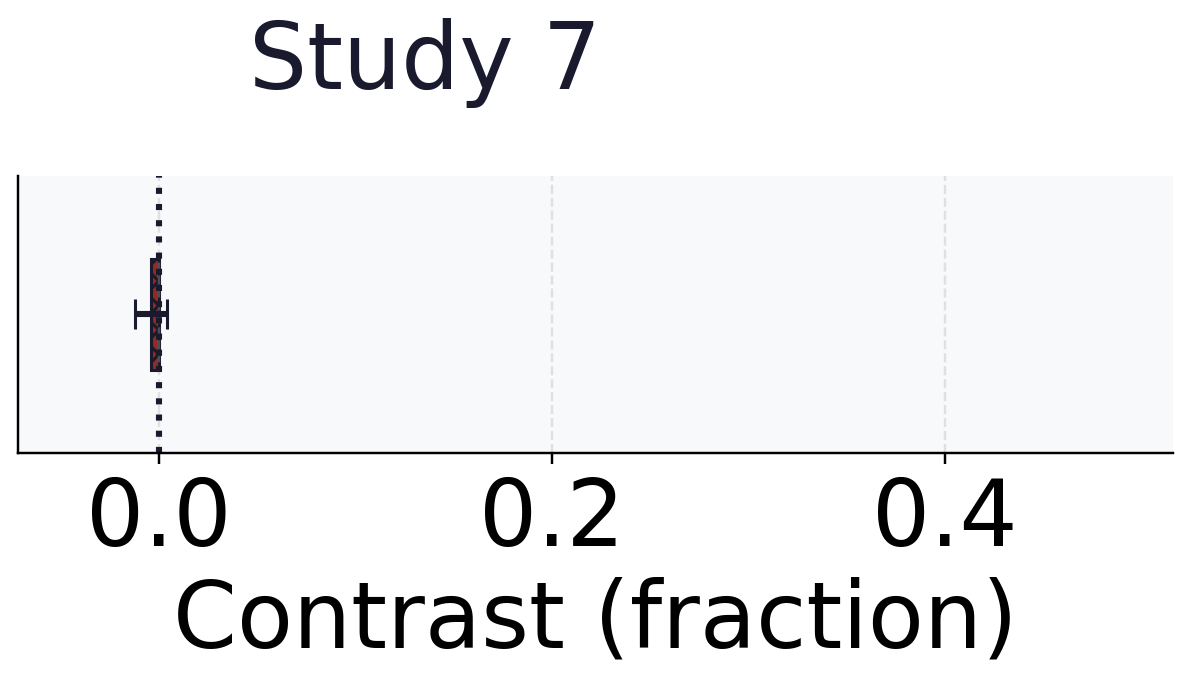
\includegraphics[keepaspectratio,width=0.98\linewidth,height=0.8\textheight,alt={Study 7
3-level hierarchical POMDP: mean and seed-bootstrap interval on the shared fraction facet scale.}]{../figures/cross_study_summary.slide-fraction-study-5.png}
\refstepcounter{figure}\label{fig:cross-study-summary-slide-panel-9}
\end{figure}
\end{frame}

\begin{frame}{Pattern 3: a conditional\ldots{} (part 40)}
\begin{figure}
\centering
\includegraphics[keepaspectratio,width=0.98\linewidth,height=0.8\textheight,alt={Study 7 3-level hierarchical POMDP. Mean -0.004297; 95\% interval {[}-0.01211, +0.003906{]} fraction.}]{../figures/cross_study_summary.slide-fraction-study-5-values.png}
\refstepcounter{figure}\label{fig:cross-study-summary-slide-panel-10}
\end{figure}
\end{frame}

\begin{frame}{Pattern 3: a conditional\ldots{} (part 41)}
\begin{figure}
\centering
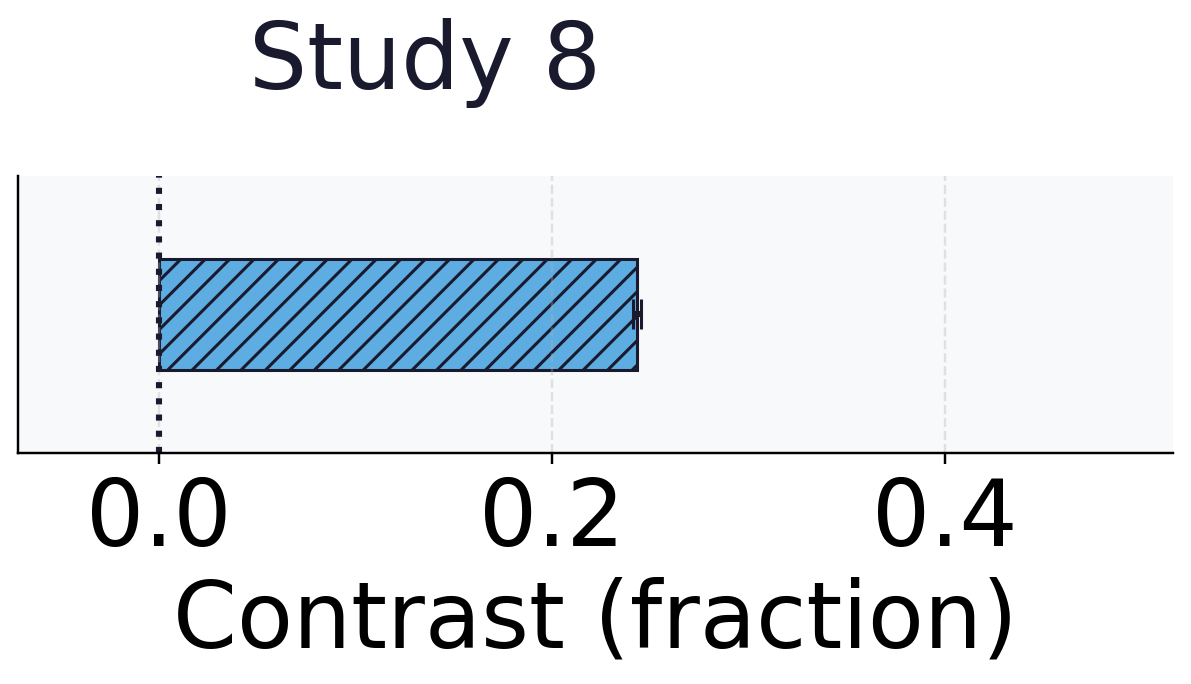
\includegraphics[keepaspectratio,width=0.98\linewidth,height=0.8\textheight,alt={Study 8
Sensitivity sweep: mean and seed-bootstrap interval on the shared fraction facet scale.}]{../figures/cross_study_summary.slide-fraction-study-6.png}
\refstepcounter{figure}\label{fig:cross-study-summary-slide-panel-11}
\end{figure}
\end{frame}

\begin{frame}{Pattern 3: a conditional\ldots{} (part 42)}
\begin{figure}
\centering
\includegraphics[keepaspectratio,width=0.98\linewidth,height=0.8\textheight,alt={Study 8 Sensitivity sweep. Mean +0.2433; 95\% interval {[}+0.2411, +0.2455{]} fraction.}]{../figures/cross_study_summary.slide-fraction-study-6-values.png}
\refstepcounter{figure}\label{fig:cross-study-summary-slide-panel-12}
\end{figure}
\end{frame}

\begin{frame}{Pattern 3: a conditional\ldots{} (part 43)}
\begin{figure}
\centering
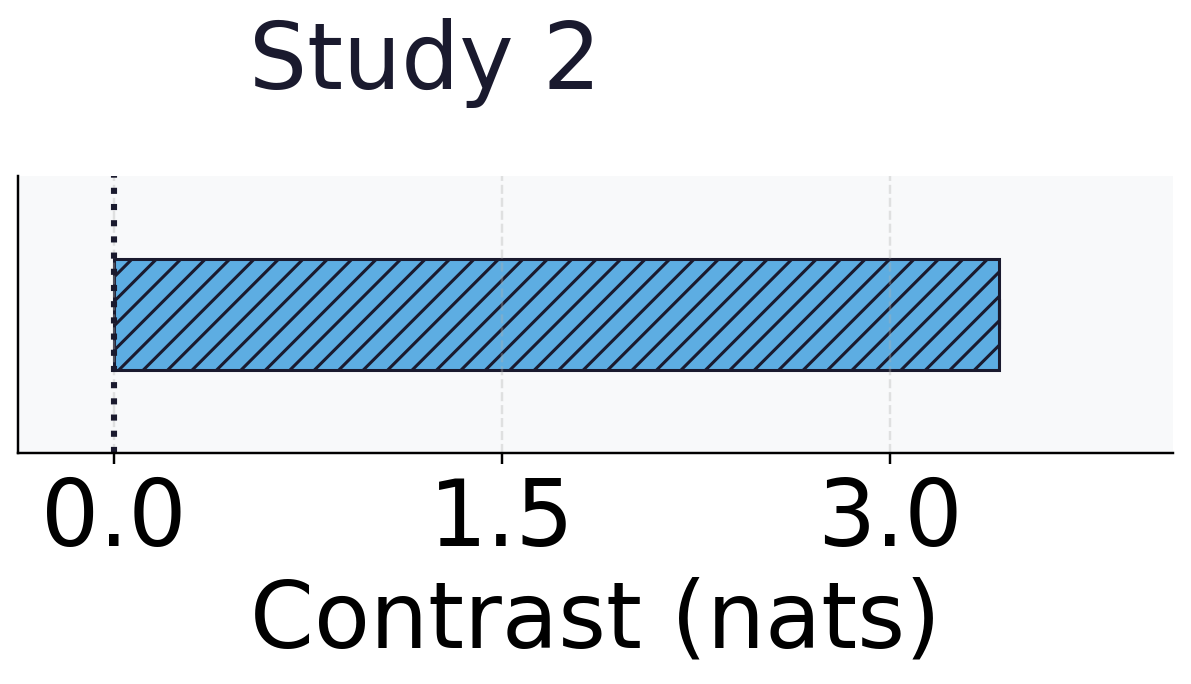
\includegraphics[keepaspectratio,width=0.98\linewidth,height=0.8\textheight,alt={Study 2
Language acquisition: mean and seed-bootstrap interval on the shared nats facet scale.}]{../figures/cross_study_summary.slide-nats-study-1.png}
\refstepcounter{figure}\label{fig:cross-study-summary-slide-panel-13}
\end{figure}
\end{frame}

\begin{frame}{Pattern 3: a conditional\ldots{} (part 44)}
\begin{figure}
\centering
\includegraphics[keepaspectratio,width=0.98\linewidth,height=0.8\textheight,alt={Study 2 Language acquisition. Mean +3.42; 95\% interval {[}+3.42, +3.421{]} nats.}]{../figures/cross_study_summary.slide-nats-study-1-values.png}
\refstepcounter{figure}\label{fig:cross-study-summary-slide-panel-14}
\end{figure}
\end{frame}

\begin{frame}{Pattern 3: a conditional\ldots{} (part 45)}
\begin{figure}
\centering
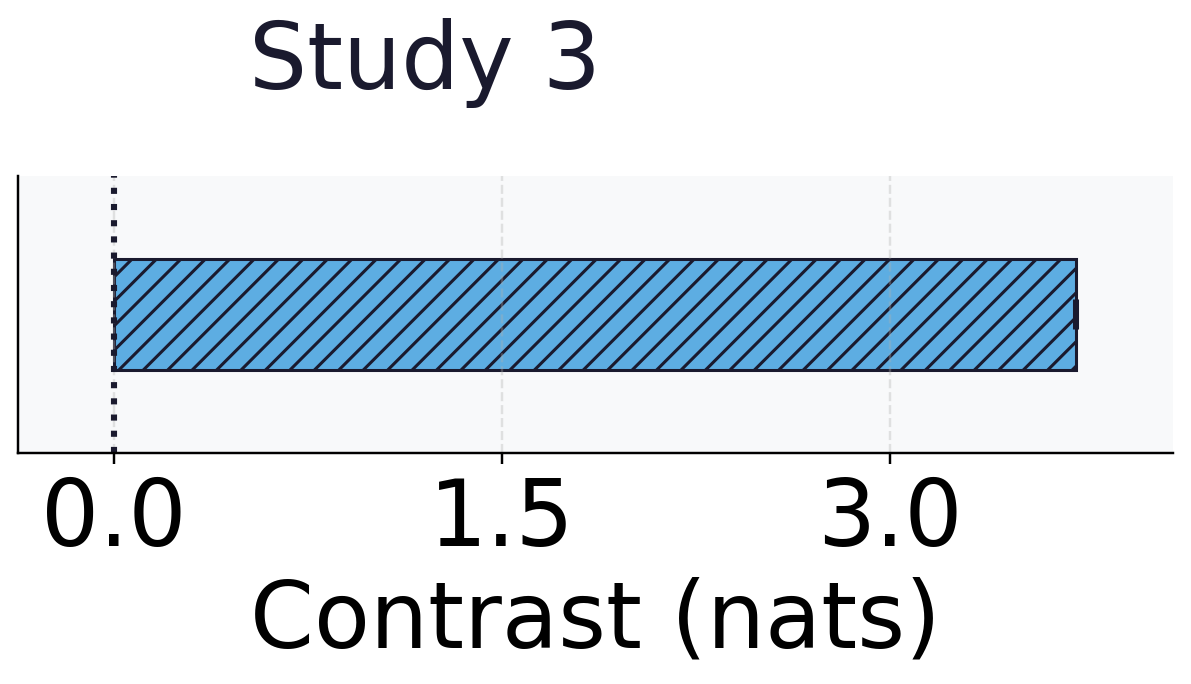
\includegraphics[keepaspectratio,width=0.98\linewidth,height=0.8\textheight,alt={Study 3
Configured BMR
sign control: mean and seed-bootstrap interval on the shared nats facet scale.}]{../figures/cross_study_summary.slide-nats-study-2.png}
\refstepcounter{figure}\label{fig:cross-study-summary-slide-panel-15}
\end{figure}
\end{frame}

\begin{frame}{Pattern 3: a conditional\ldots{} (part 46)}
\begin{figure}
\centering
\includegraphics[keepaspectratio,width=0.98\linewidth,height=0.8\textheight,alt={Study 3 Configured BMR sign control. Mean +3.716; 95\% interval {[}+3.71, +3.722{]} nats.}]{../figures/cross_study_summary.slide-nats-study-2-values.png}
\refstepcounter{figure}\label{fig:cross-study-summary-slide-panel-16}
\end{figure}
\end{frame}

\begin{frame}{Pattern 3: a conditional\ldots{} (part 47)}
\begin{figure}
\centering
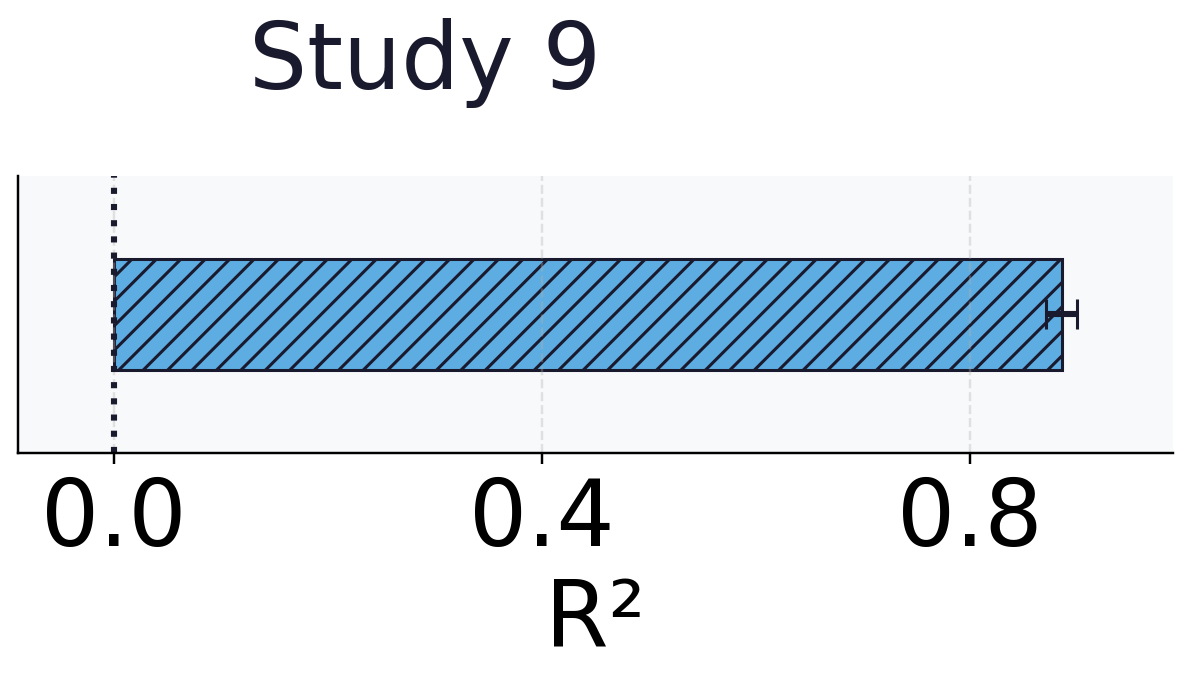
\includegraphics[keepaspectratio,width=0.98\linewidth,height=0.8\textheight,alt={Study 9
Parameter recovery: mean and seed-bootstrap interval on the shared R-sq facet scale.}]{../figures/cross_study_summary.slide-rsq-study-1.png}
\refstepcounter{figure}\label{fig:cross-study-summary-slide-panel-17}
\end{figure}
\end{frame}

\begin{frame}{Pattern 3: a conditional\ldots{} (part 48)}
\begin{figure}
\centering
\includegraphics[keepaspectratio,width=0.98\linewidth,height=0.8\textheight,alt={Study 9 Parameter recovery. Mean +0.8861; 95\% interval {[}+0.8716, +0.9005{]} R-sq.}]{../figures/cross_study_summary.slide-rsq-study-1-values.png}
\refstepcounter{figure}\label{fig:cross-study-summary-slide-panel-18}
\end{figure}
\end{frame}

\begin{frame}{Pattern 3: a conditional\ldots{} (part 49)}
\begin{figure}
\centering
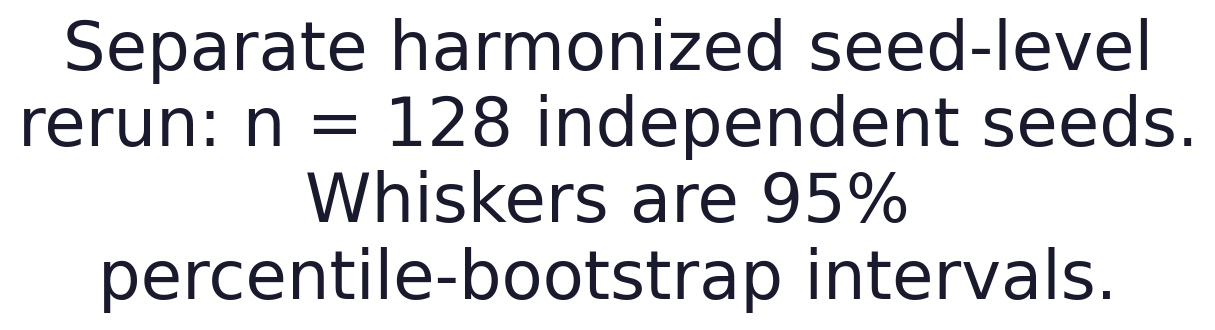
\includegraphics[keepaspectratio,width=0.98\linewidth,height=0.8\textheight,alt={Separate harmonized seed-level rerun: n = 128 independent seeds. Whiskers are 95\% percentile-bootstrap intervals.}]{../figures/cross_study_summary.slide-uncertainty.png}
\refstepcounter{figure}\label{fig:cross-study-summary-slide-panel-19}
\end{figure}
\end{frame}

\begin{frame}{Pattern 3: a conditional\ldots{} (part 50)}
\begin{figure}
\centering
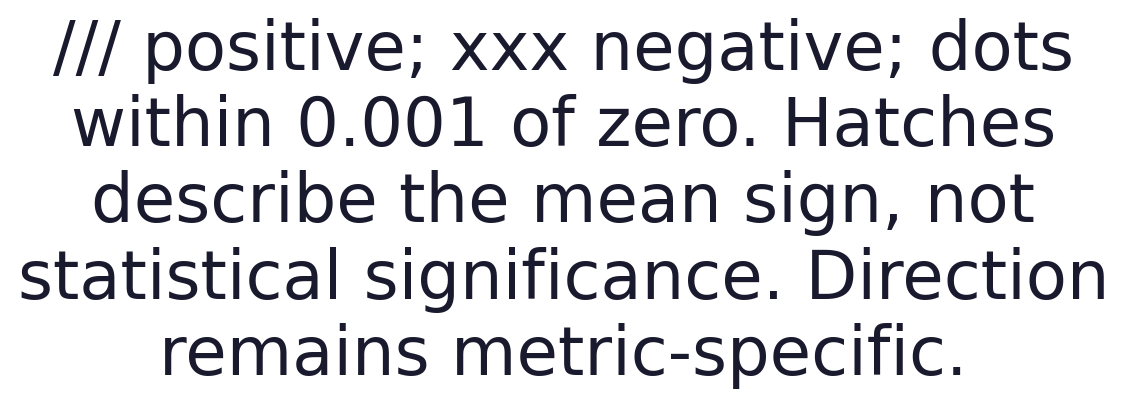
\includegraphics[keepaspectratio,width=0.98\linewidth,height=0.8\textheight,alt={/// positive; xxx negative; dots within 0.001 of zero. Hatches describe the mean sign, not statistical significance. Direction remains metric-specific.}]{../figures/cross_study_summary.slide-direction.png}
\refstepcounter{figure}\label{fig:cross-study-summary-slide-panel-20}
\end{figure}
\end{frame}

\begin{frame}{Pattern 3: a conditional\ldots{} (part 51)}
\begin{figure}
\centering
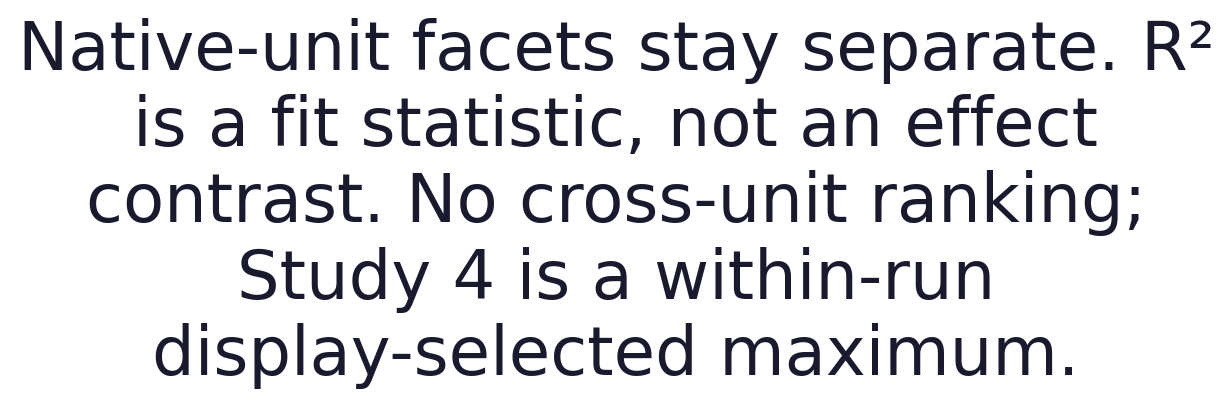
\includegraphics[keepaspectratio,width=0.98\linewidth,height=0.8\textheight,alt={Native-unit facets stay separate. R² is a fit statistic, not an effect contrast. No cross-unit ranking; Study 4 is a within-run display-selected maximum.}]{../figures/cross_study_summary.slide-scope.png}
\refstepcounter{figure}\label{fig:cross-study-summary-slide-panel-21}
\end{figure}
\end{frame}

\end{document}
